\documentclass[11pt, oneside]{book}   		% Allgemeine Schriftgröße, Dokumententyp
%!TEX root=../Vorlage_DA.tex
%	%%%%%%%%%%%%%%%%%%%%%%%%%%%%%%%%%%%%%%%%%%%%%%%%%%%%%%%%
% 	Packages
%	%%%%%%%%%%%%%%%%%%%%%%%%%%%%%%%%%%%%%%%%%%%%%%%%%%%%%%%%
\usepackage{geometry}                		
\usepackage{german}
\usepackage{ngerman}
\usepackage[parfill]{parskip}    			% Activate to begin paragraphs with an empty line rather than an indent
\usepackage{graphicx}						% Use pdf, png, jpg, or epsß with pdflatex; use eps in DVI mode
											% TeX will automatically convert eps --> pdf in pdflatex		

%\usepackage{helvet}						% Kommentar wegnehmen, um in Helvetica zu schreiben
%\renewcommand{\familydefault}{\sfdefault}
%\fontfamily{phv}\selectfont
								
\usepackage{amssymb}
\usepackage[utf8]{inputenc}


\usepackage{geometry}
\usepackage{tabularx}
\usepackage{multirow}
\usepackage{arydshln}
\usepackage{subfig}

\usepackage{forloop}								
\usepackage{listings}
\usepackage{color} 
\usepackage{colortbl}
\usepackage{courier}
\usepackage{pifont}

\usepackage[pdftex]{hyperref}
\usepackage{url}


%	%%%%%%%%%%%%%%%%%%%%%%%%%%%%%%%%%%%%%%%%%%%%%%%%%%%%%%%%
% 	Dokumentabmessungen, Farbdefinitionen	
%	%%%%%%%%%%%%%%%%%%%%%%%%%%%%%%%%%%%%%%%%%%%%%%%%%%%%%%%%
%\geometry {a4paper, left=22mm, right=22mm, top=25mm, bottom=25mm, landscape}
\geometry {a4paper, bottom=30mm}%, left=30mm, right=30mm, top=25mm, bottom=25mm}
\pagestyle{headings}

\definecolor{grey}{RGB}{127,127,127}
\definecolor{lightgrey}{RGB}{180,180,180}
\definecolor{dkgreen}{rgb}{0,0.6,0}  
\definecolor{gray}{rgb}{0.5,0.5,0.5} 
\definecolor{mauve}{rgb}{0.58,0,0.82}


\definecolor{cssId}{rgb}		{0,0,0.6 }%{0.75, 0.00, 0.00 }
\definecolor{cssAttribute}{rgb}	{0.58,0,0.82 }%{0.00, 0.00, 0.75 }
\definecolor{cssClass}{rgb}		{0,0,0.6 }%{0.00, 0.75, 0.00 }
\definecolor{cssComment}{rgb}	{0,0.6,0 }%{0.00, 0.75, 0.00 }
\definecolor{cssString}{rgb}	{0.6,0,0 }%{0.00, 0.75, 0.00 }



%	%%%%%%%%%%%%%%%%%%%%%%%%%%%%%%%%%%%%%%%%%%%%%%%%%%%%%%%%
% 	Diverse Befehle		
%	%%%%%%%%%%%%%%%%%%%%%%%%%%%%%%%%%%%%%%%%%%%%%%%%%%%%%%%%

%	Quelltext im Textfluss
\def\inlinecode#1{\texttt{\color{gray}{#1}}}


%	Paragraph mit Zeilenumbruch nachher
\def\htlParagraph#1{\paragraph*{#1}$\;$ \\}



%	%%%%%%%%%%%%%%%%%%%%%%%%%%%%%%%%%%%%%%%%%%%%%%%%%%%%%%%%
% 	Code Formatierung		
%	%%%%%%%%%%%%%%%%%%%%%%%%%%%%%%%%%%%%%%%%%%%%%%%%%%%%%%%%
\lstset{literate=%
{Ö}{{\"O}}1 
{Ä}{{\"A}}1 
{Ü}{{\"U}}1 
{ß}{{\ss}}2 
{ü}{{\"u}}1 
{ä}{{\"a}}1 
{ö}{{\"o}}1
}
 
\lstset{ % 
%  language=Octave,                			% the language of the code 
%  basicstyle=\footnotesize,           		% the size of the fonts that are used for the code 
 	basicstyle=\ttfamily, ,           		% the size of the fonts that are used for the code 
	numbers=left,                   		% where to put the line-numbers 
	numberstyle=\tiny\color{gray},  		% the style that is used for the line-numbers 
	stepnumber=1,                   		% the step between two line-numbers. If it's 1, each line  
                                  			% will be numbered 
	numbersep=5pt,                  		% how far the line-numbers are from the code 
	backgroundcolor=\color{white},    	  	% choose the background color. You must add \usepackage{color}
	showspaces=false,               		% show spaces adding particular underscores 
	showstringspaces=false,      	   		% underline spaces within strings
	showtabs=false,                 		% show tabs within strings adding particular underscores
%	frame=single,                   		% adds a frame around the code
	frame=l,
	rulecolor=\color{dkgreen},        		% if not set, the frame-color may be changed on line-breaks within not-black text (e.g. comments (green here))
	tabsize=2,                      		% sets default tabsize to 2 spaces
	captionpos=b,                   		% sets the caption-position to bottom
	breaklines=true,                		% sets automatic line breaking
	breakatwhitespace=false,        		% sets if automatic breaks should only happen at whitespace
%	title=\lstname,                   		% show the filename of files included with \lstinputlisting;
          	                        		% also try caption instead of title
	keywordstyle=\color{blue},          	% keyword style
	commentstyle=\color{dkgreen},       	% comment style
	stringstyle=\color{mauve},    	     	% string literal style
	escapeinside={\%*}{*)},            		% if you want to add LaTeX within your code
	morekeywords={*,...},              		% if you want to add more keywords to the set
	deletekeywords={...}             	 	% if you want to delete keywords from the given language
}

%	%%%%%%%%%%%%%%%%%%%%%%%%%%%%%%%%%%%%%%%%%%%%%%%%%%%%%%%%
% 	CSS		
\lstdefinelanguage{CSS}{
		alsoletter={\\,/,*,:,-,\#,.},
		identifierstyle=\idstyle,
        keywords={accelerator:, azimuth:, background:, background-attachment:, background-color:, background-image:, background-position:, background-position-x:, background-position-y:, background-repeat:, behavior:, border:, border-bottom:, border-bottom-color:, border-bottom-style:, border-bottom-width:, border-collapse:, border-color:, border-left:, border-left-color:, border-left-style:, border-left-width:, border-right:, border-right-color:, border-right-style:, border-right-width:, border-spacing:, border-style:, border-top:, border-top-color:, border-top-style:, border-top-width:, border-width:, bottom   :, caption-side:, clear:, clip:, color:, content:, counter-increment:, counter-reset:, cue:, cue-after:, cue-before:, cursor:, direction:, display:, elevation:, empty-cells :, filter:, float:, font:, font-family:, font-size:, font-size-adjust:, font-stretch:, font-style:, font-variant:, font-weight:, height:, ime-mode:, include-source:, layer-background-color:, layer-background-image:, layout-flow:, layout-grid:, layout-grid-char:, layout-grid-char-spacing:, layout-grid-line:, layout-grid-mode:, layout-grid-type:, left:, letter-spacing:, line-break:, line-height:, list-style:, list-style-image:, list-style-position:, list-style-type:, margin:, margin-bottom:, margin-left:, margin-right:, margin-top:, marker-offset:, marks:, max-height:, max-width:, min-height:, min-width:, -moz-binding:, -moz-border-radius:, -moz-border-radius-topleft:, -moz-border-radius-topright:, -moz-border-radius-bottomright:, -moz-border-radius-bottomleft:, -moz-border-top-colors:, -moz-border-right-colors:, -moz-border-bottom-colors:, -moz-border-left-colors:, -moz-opacity:, -moz-outline:, -moz-outline-color:, -moz-outline-style:, -moz-outline-width:, -moz-user-focus:, -moz-user-input:, -moz-user-modify:, -moz-user-select:, orphans:, outline:, outline-color:, outline-style:, outline-width:, overflow:, overflow-X:, overflow-Y:, padding:, padding-bottom:, padding-left:, padding-right:, padding-top:, page:, page-break-after:, page-break-before:, page-break-inside:, pause:, pause-after:, pause-before:, pitch:, pitch-range:, play-during:, position:, quotes:, -replace:, richness:, right:, ruby-align:, ruby-overhang:, ruby-position:, -set-link-source:, size:, speak:, speak-header:, speak-numeral:, speak-punctuation:, speech-rate:, stress:, scrollbar-arrow-color:, scrollbar-base-color:, scrollbar-dark-shadow-color:, scrollbar-face-color:, scrollbar-highlight-color:, scrollbar-shadow-color:, scrollbar-3d-light-color:, scrollbar-track-color :, table-layout:, text-align:, text-align-last:, text-decoration:, text-indent:, text-justify:, text-overflow:, text-shadow:, text-transform:, text-autospace:, text-kashida-space:, text-underline-position:, top:, unicode-bidi:, -use-link-source:, vertical-align:, visibility:, voice-family:, volume :, white-space:, widows:, width:, word-break:, word-spacing:, word-wrap:, writing-mode},
        keywordstyle=\color{cssAttribute},%\bfseries,
        ndkeywords={@import, @media, @page, @font-face, @charset, @namespace, a, html, body, title, pre, h1, h2, h3, h4, h5, h6, ul, ol, li, p, br, blockquote, dl, dt, dd, div, img, strong, em, cite, tt, i, b, table, tr, td, th, frame, form, option, input, button, nav, section, article, aside, footer, hr, sup, sub, del, ins, small, span},
        ndkeywordstyle=\color{cssId},%,\bfseries,
%        identifierstyle=\color{black},
%        sensitive=false,
%        comment=[l]{//},
        morecomment=[s]{/*}{*/},
        commentstyle=\color{cssComment}\ttfamily,
        stringstyle=\color{cssString}\ttfamily,
        morestring=[b]',
        morestring=[b]"
}

\makeatletter
\newcommand*\idstyle[1]{%
         \expandafter\id@style\the\lst@token{#1}\relax%
 }

 \def\id@style#1#2\relax{%
           	\ifnum\pdfstrcmp{#1}{\#}=0%
                \small\ttfamily\color{cssId} \the\lst@token%
            \else%
		      	\ifnum\pdfstrcmp{#1}{.}=0%
    	            \small\ttfamily\color{cssClass} \the\lst@token%
        		\else%
					\ifnum\pdfstrcmp{#1}{:}=0%
    	            	\small\ttfamily\color{cssAttribute} \the\lst@token%
        			\else%
		     	 		\edef\tempa{\uccode`#1}%
              			\edef\tempb{`#1}%
              			\ifnum\tempa=\tempb%
                			\small\ttfamily\color{mauve} \the\lst@token%
              			\else%
                 	 		\the\lst@token%
    	         		\fi%
	           		\fi%
	            \fi%
            \fi%
 }
\makeatother


%	%%%%%%%%%%%%%%%%%%%%%%%%%%%%%%%%%%%%%%%%%%%%%%%%%%%%%%%%
% 	EBNF	
\lstdefinelanguage{EBNF}{
        keywords={},
		alsoletter={\{,\}\\,/,*,:,-,\#,.},
        comment=[l]{//},
        morecomment=[s]{/*}{*/},
        morestring=[b]',
        morestring=[b]"
}		% Formatierung der Dokuments, Diverse Befehle


%	########################################################
% 					Allgemeine Informationen			
%	########################################################
\def\htlArbeit{Diplomarbeit }
\def\htlArbeitsthema{\LaTeX -Vorlage für eine \htlArbeit}	% Thema oder Titel der Arbeit
\def\htlArbeitstitel{Arbeitstitel für das Projekt }			% Arbeitstitel


\begin{document}

%	########################################################
% 						Einleitung			
%	########################################################
\pagenumbering{roman}	% Beginn mit römischen Seitenzahlen

%	--------------------------------------------------------
% 	Deckblatt
%	--------------------------------------------------------			
%!TEX root=../Vorlage_DA.tex
%	########################################################
% 							Deckblatt
%	########################################################

\newgeometry{top=1cm}
\begin{titlepage}
\title{
%
{
\includegraphics[width=0.15\textwidth]{./includes/htl_c_cmyk_rein.pdf}}
%
\\{\normalsize \textbf{Höhere Technische Bundeslehranstalt}}
\\[-0.4em] {\normalsize \textbf{und Bundesfachschule}}
\\[-0.4em] {\normalsize im Hermann Fuchs Bundesschulzentrum}
%
\\\vspace{3cm}{ \textbf{\htlArbeitsthema}}
%
\\\vspace{0.5cm} {\Large \textsc{\htlArbeit}}
%
\\\vspace{5cm}
%
{\normalsize \emph{Ausgeführt im Schuljahr 2012/2013 von:}}
\\{\normalsize Max Mustermann, 5BHELS}
\\[-0.4em] {\normalsize Frieda Fröhlich, 5BHELS}
\\[1.0em] {\normalsize \emph{Betreuer:}}
\\{\normalsize Dipl.-Ing. Lukas Lämpel}
}		
%
\maketitle
\end{titlepage}
\restoregeometry
\pagebreak


%	--------------------------------------------------------
% 	Arbeitstitel
%	--------------------------------------------------------		
%!TEX root=../Vorlage_DA.tex
%	########################################################
% 							Arbeitstitel
%	########################################################


%	--------------------------------------------------------
% 	Überschrift, Inhaltsverzeichnis
%	--------------------------------------------------------
\chapter*{Arbeitstitel: \newline \htlArbeitstitel}



%	--------------------------------------------------------
% 	Bearbeiter
%	--------------------------------------------------------
\htlParagraph{Bearbeiter: Fabian Hummer}


%	--------------------------------------------------------
% 	Beteiligte Firmen
%	--------------------------------------------------------
\htlParagraph{An der \htlArbeit beteiligte Firmen:}

\renewcommand{\arraystretch}{1.5}
\begin{tabularx}{1\textwidth}{@{} l X @{}}

\emph{Firma:} & Institut für Systemsoftware\newline Johannes Kepler Universität Linz\\
\emph{Adresse:} & Altenbergstraße, 69\\
\emph{Plz, Ort:} & 4040, Linz\\
\emph{Kontaktperson:} & Prof. Dr. Dr. h.c. Hanspeter Mössenböck\\
\emph{Telefon:} & + 43-732-2468-4340\\
\emph{E-Mail:} & moessenboeck@ssw.uni-linz.at\\

\end{tabularx}


%	--------------------------------------------------------
% 	Eidesstattliche Erklärung
%	--------------------------------------------------------			
%!TEX root=../Vorlage_DA.tex
%	########################################################
% 					Eidesstattliche Erklärung
%	########################################################


%	--------------------------------------------------------
% 	Überschrift, Inhaltsverzeichnis
%	--------------------------------------------------------
\chapter*{Erklärung}
\addcontentsline{toc}{chapter}{Erklärung}


%	--------------------------------------------------------
% 	Inhalt
%	--------------------------------------------------------

Ich erkläre an Eides statt, dass ich die vorliegende Diplomarbeit selbstständig und ohne fremde Hilfe verfasst, andere als angegebene Quellen und Hilfsmittel nicht direkt benutzt und die benutzten Quellen wörtlich und inhaltlich entnommenen Stellen als solche erkenntlich gemacht habe.
\vspace{3cm}

\begin{tabularx}{1\textwidth}{X p{1cm} X p{1cm} X}


\hrulefill & & \hrulefill & & \hrulefill \\
\emph{Ort, Datum} & & \emph{Verfasser Vor- und Zunamen} & & \emph{Unterschrift/en}
\end{tabularx}




%	--------------------------------------------------------
% 	Inhaltsverzeichnis
%	--------------------------------------------------------			
\tableofcontents

%	--------------------------------------------------------
% 	Vorwort
%	--------------------------------------------------------	
%%!TEX root=../Vorlage_DA.tex
%	########################################################
% 							Vorwort
%	########################################################


%	--------------------------------------------------------
% 	Überschrift, Inhaltsverzeichnis
%	--------------------------------------------------------
\chapter*{Vorwort}
\addcontentsline{toc}{chapter}{Vorwort}


%	--------------------------------------------------------
% 	Inhalt
%	--------------------------------------------------------

Im Vorwort teilt der Bearbeiter dem Leser wichtige Tatsachen mit, die Erklärungen zu seiner Arbeit beinhalten -- z.B. die Motivation für die Bearbeitung des Themas oder besondere Schwierigkeiten bei der Bearbeitung und/oder Materialbeschaffung. 

Hier können auch Mitteilungen persönlicher Natur enthalten sein -- z.B. Dank an Institutionen/Personen für die geleistete Unterstützung. 

%	--------------------------------------------------------
% 	Zusammenfassung
%	--------------------------------------------------------		
%%!TEX root=../Vorlage_DA.tex
%	########################################################
% 							Zusammenfassung
%	########################################################


%	--------------------------------------------------------
% 	Überschrift, Inhaltsverzeichnis
%	--------------------------------------------------------
\chapter*{Zusammenfassung}
\addcontentsline{toc}{chapter}{Zusammenfassung}



%	--------------------------------------------------------
% 	Inhalt
%	--------------------------------------------------------
Die \emph{Zusammenfassung} oder auch \emph{Kurzfassung} soll der Inhalt der \htlArbeit auf maximal einer halben Seite zusammengefasst werden.

%	--------------------------------------------------------
% 	Abstract
%	--------------------------------------------------------		
%%!TEX root=../Vorlage_DA.tex
%	########################################################
% 							Abstract
%	########################################################


%	--------------------------------------------------------
% 	Überschrift, Inhaltsverzeichnis
%	--------------------------------------------------------
\chapter*{Abstract}
\addcontentsline{toc}{chapter}{Abstract}



%	--------------------------------------------------------
% 	Inhalt
%	--------------------------------------------------------
The \emph{abstract} is the english version of the \emph{Kurzfassung}. The  \emph{abstract} should not be any longer than one half of a page.



%	########################################################
% 						Arbeit			
%	########################################################

%	--------------------------------------------------------
% 	INFO: Zitieren, Abbildungen, Listing
%	-------------------------------------------------------	
%%!TEX root=../Vorlage_DA.tex
%	########################################################
% 			INFO: Zitieren, Abbildungen, Listing
%	########################################################


%	--------------------------------------------------------
% 	Überschrift, Inhaltsverzeichnis
%	--------------------------------------------------------
\chapter*{INFO: Zitieren, Abbildungen, Listing}

In diesem Kapitel sind Beispiele angeführt, wie Abbildungen, Zitate und Quelltext zu verwenden sind.

Die Zitate und die Abbildungen werden automatisch in das Quellen- und Abbildungsverzeichnis übernommen. Das Quellenverzeichnis und das Abbildungsverzeichnis sind am Ende der Arbeit zu finden.   

\textbf{Beispiel: Icons--Beschreibung}
\setlength{\extrarowheight}{0.1cm}

\begin{tabularx}{\textwidth}{p{1.2cm} | X }

\vspace{-0.4cm}
\includegraphics[width=1cm]{./media/images/htl_c_cmyk_rein.pdf} & Hier kommt dann die Beschreibung zum Icon dazu. Wenn es über mehrer Zeilen gehen sollte, dann erfolgt das mit dem \LaTeX--Befehl \inlinecode{newline}. 
\newline Hier geht die Beschreibung dann weiter \ldots
\\ 
\vspace{-0.4cm}
\includegraphics[width=1cm]{./media/images/htl_c_cmyk_rein.pdf} & Hier kommt dann die Beschreibung zum Icon dazu. Wenn es über mehrer Zeilen gehen sollte, dann erfolgt das mit dem \LaTeX--Befehl \inlinecode{newline}. 
\newline Hier geht die Beschreibung dann weiter \ldots
\\
\vspace{-0.4cm}
\includegraphics[width=1cm]{./media/images/htl_c_cmyk_rein.pdf} & Hier kommt dann die Beschreibung zum Icon dazu. Wenn es über mehrer Zeilen gehen sollte, dann erfolgt das mit dem \LaTeX--Befehl \inlinecode{newline}. 
\newline Hier geht die Beschreibung dann weiter \ldots
\\
\vspace{-0.4cm}
\includegraphics[width=1cm]{./media/images/htl_c_cmyk_rein.pdf} & Hier kommt dann die Beschreibung zum Icon dazu. Wenn es über mehrer Zeilen gehen sollte, dann erfolgt das mit dem \LaTeX--Befehl \inlinecode{newline}. 
\newline Hier geht die Beschreibung dann weiter \ldots


\end{tabularx}


%	--------------------------------------------------------
% 	Inhalt 
%	--------------------------------------------------------
\section*{Abbildungen}


In der Abbildung \ref{htl01} auf Seite \pageref{htl01} ist das Logo der HTL im Farbmodus \emph{CMYK} zu sehen. Das Logo ist im \emph{.pdf}-Format gespeichert und setzt sich ausschließlich aus Pfaden zusammen.

%	--------------
%	Eine Abbildung
\begin{figure}[t]
	\centering
	
\includegraphics[width=0.5\textwidth]{./media/images/htl_c_cmyk_rein.pdf}
  	\caption{Logo der HTL Braunau.}
  	\label{htl01}
\end{figure}


%	----------------
%	Zwei Abbildungen

\begin{figure}[bht]
  \centering
  \subfloat[Logo der HTL Braunau.]{\label{fig:a}
\includegraphics[width=.4\textwidth]{./media/images/htl_c_cmyk_rein.pdf}}
  \qquad
  \subfloat[Logo der HTL Braunau.]{\label{fig:b}
\includegraphics[width=.4\textwidth]{./media/images/htl_c_cmyk_rein.pdf}}
  \label{fig:canvas_01}
\caption[]{Zwei Logos der HTL Braunau mit in einer Abbildung zusammengefasst.}
\end{figure}


%	----------------
%	Drei Abbildungen
\begin{figure}[htb]
  \centering
  \subfloat[Logo der HTL Braunau.]{\label{fig:a}
\includegraphics[width=.29\textwidth]{./media/images/htl_c_cmyk_rein.pdf}}
  \qquad
  \subfloat[Logo der HTL Braunau.]{\label{fig:b}
\includegraphics[width=.29\textwidth]{./media/images/htl_c_cmyk_rein.pdf}}
\qquad
  \subfloat[Logo der HTL Braunau.]{\label{fig:b}
\includegraphics[width=.29\textwidth]{./media/images/htl_c_cmyk_rein.pdf}}
  \label{fig:canvas_04}
\caption[]{Die Reihenfolge der Transformationen wirkt sich auf die Transformationsmatrix aus.}
\end{figure}


\section*{Zitate, Fußnoten, Literaturverzeichnis}

Die einzelnen Quellen sind in einer eigenen Datei hinterlegt. Konkret ist es bei diesem Dokument die Datei \href{"./includes/literatur.bib"}{\emph{literatur.bib}}, die sich im Verzeichnis \emph{includes} befindet.

Man sollte immer höflich bleiben ~\cite{autor:01}.\\

Wörtliche Zitate werden durch Anführungszeichen begonnen und beendet und kursiv geschrieben: \emph{\glqq We tend to think of navigating a website as clicking from page-to-page via some kind of global navigation that’s always visible. When it comes to a single page, we often think scrolling is the one and only way to move from one end to the next.\grqq}~\cite{smashing:01}.


Es ist zunehmend eine Kurzzitierweise in Fußnoten üblich: Nachname des Verfassers, Kurztitel, Seitenangabe.\footnote{John Doe, \glqq Verwendung von Fußnoten\grqq, Seite 12.}


%	%%%%%%%%%%%%%%%%%%%%%%%%%%%%%%%%%%%%%%%%%%%%%
%	Listings, Code
%	%%%%%%%%%%%%%%%%%%%%%%%%%%%%%%%%%%%%%%%%%%%%%
\section*{Listings, Code}
Wie aus dem Quelltext \ref{code01} auf Seite \pageref{code01} hervorgeht, \ldots


%	%%%%%%%%%%%%%%%%%%%%%%%%%%%%%%%%%%%%%%%%%%%%%
%	C++
\begin{figure}[H]
	\lstinputlisting[language=C++]{./media/code_snippets/bsp_01.cpp}
	\caption{Mein ersters C-Programm.}
  	\label{code01}
\end{figure}


%	%%%%%%%%%%%%%%%%%%%%%%%%%%%%%%%%%%%%%%%%%%%%%
%	CSS
\begin{figure}[H]
	\lstinputlisting[language=CSS]{./media/code_snippets/bsp.css}
	\caption{Kurzer CSS--Quelltext.}
  	\label{code02}
\end{figure}

%	%%%%%%%%%%%%%%%%%%%%%%%%%%%%%%%%%%%%%%%%%%%%%
%	HTML
\begin{figure}[H]
	\lstinputlisting[language=HTML]{./media/code_snippets/bsp.html}
	\caption{HTML--Quelltext}
  	\label{code03}
\end{figure}


%	%%%%%%%%%%%%%%%%%%%%%%%%%%%%%%%%%%%%%%%%%%%%%
%	HTML
\begin{figure}[H]
	\lstinputlisting[language=JavaScript]{./media/code_snippets/bsp.js}
	\caption{JavaScript--Quelltext}
  	\label{code04}
\end{figure}

%	%%%%%%%%%%%%%%%%%%%%%%%%%%%%%%%%%%%%%%%%%%%%%
%	Listings direkt im Programmfluss
Text vor einem Quelltext--Block \ldots

\begin{lstlisting}[language=CSS]
#idStyle.class {
	background-color: red;
	color: white;
}

.classStyle {
	color: blue;
}
\end{lstlisting}

\ldots Text nach einem Quelltext--Block.


\begin{lstlisting}[language=TypoScript]
10.
\end{lstlisting}

 	% Nur zur Info

%	--------------------------------------------------------
% 	Aufgabenstellung / Pflichtenheft
%	--------------------------------------------------------		
%%!TEX root=../Vorlage_DA.tex
%	########################################################
% 				Aufgabenstellung/Pflichtenheft
%	########################################################


%	--------------------------------------------------------
% 	Überschrift, Inhaltsverzeichnis
%	--------------------------------------------------------
\chapter{Aufgabenstellung/Pflichtenheft}


%	--------------------------------------------------------
% 	Section 1
%	--------------------------------------------------------
\section{Section 1}

\pagenumbering{arabic}	% Beginn mit arabischen Seitenzahlen

%	--------------------------------------------------------
% 	Compiler
%	--------------------------------------------------------	
%!TEX root=../Vorlage_DA.tex
%	########################################################
% 				Projektbeschreibung
%	########################################################


%	--------------------------------------------------------
% 	Überschrift, Inhaltsverzeichnis
%	--------------------------------------------------------
\chapter{Compiler}

%	--------------------------------------------------------
% 	Allgmeine Hinweise
%	--------------------------------------------------------
%!TEX root=../Vorlage_DA.tex
%	########################################################
% 				Allgemeiner Teil (Theorie)
%	########################################################


%	--------------------------------------------------------
% 	Allgmeine Hinweise
%	--------------------------------------------------------
\section{Allgemeiner Teil (Theorie)}

\subsection{Erweiterte Backus-Naur-Form (EBNF)}

Die sogenannte Erweiterte Backus-Naur-Form (EBNF)\footnote{\url{https://de.wikipedia.org/wiki/Erweiterte_Backus-Naur-Form}} ist eine weiterentwicklung der Backus-Naur-Form (BNF)\footnote{\url{https://de.wikipedia.org/wiki/Backus-Naur-Form}}. Das Anwendungsgebiet der BNF und EBNF ist das definieren von  kontextfreie Grammatiken\footnote{\url{https://de.wikipedia.org/wiki/Kontextfreie_Grammatik}}, welche untere anderem f\"ur Programmiersprachen benutzt werden.

Bei kontextfreier Gramatik wird jeweils Ein Nichtterminalsymbol auf eine beliebige Folge von Terminal- bzw. Nichtterminalsymbolen abgeleitet ($V \rightarrow w$). Wenn das Nichtterminalsymbol $V$ in einem anderem Nichtterminalsymbol verwendet wird, wird nicht auf den Kontext geachtet, in welcher das Nichtterminalsymbol $V$ eingebettet ist. Die Regel ist daher kontextfrei.

Vorteile der EBNF gegen\"uber der BNF sind unter anderem:

\begin{itemize}
  \item einfacheres erstellen von Rekursionen und optionalen Ausdr\"ucken
  \item bessere Lesbarkeit
  \item einfaches und eindeutiges Definieren von Terminalsymbolen
\end{itemize}

\newpage

\subsubsection{Terminalsymbol}

Ein sogenanntes Terminalsymbol\footnote{\url{https://de.wikipedia.org/wiki/Terminalsymbol}} wird nicht weiter zerlegt. Es stellt z.B. eine Zahl, eine Variable oder ein Schlüsselwort (''if'', ''while'', ...) dar.

\begin{lstlisting}[language=EBNF]
Expr = Term { ( "+" | "-" ) Term }.
Term = intCon { ( "*" | "/" ) intCon }.
\end{lstlisting}

Terminalsymbole werden normalerweise entweder klein geschrieben (z.B. intCon), oder direkt in der Gramatik definiert (z.B. ''+'').

\subsubsection{Nichtterminalsymbol}

Ein Nichtterminalsymbol\footnote{\url{https://de.wikipedia.org/wiki/Nichtterminalsymbol}} besteht aus einen oder mehreren Terminalsymbolen bzw. Nichtterminalsymbolen.

\begin{lstlisting}[language=EBNF]
Expr = Term { ( "+" | "-" ) Term }.
Term = intCon { ( "*" | "/" ) intCon }.
\end{lstlisting}

Nichtterminalsymbole werden normalerweise gro\ss{} geschrieben. In diesem Beispiel stellen ''Expr'' und ''Term'' Nichtterminalsymbole dar, welche wiederum von anderen Nichtterminalsymbolen verwendet werden k\"onnen.

\subsubsection{Produktionsregel}

Die Produktionsregel\footnote{\url{https://de.wikipedia.org/wiki/Produktionsregel}} ist eine Regel, welche angibt wie aus W\"ortern neue W\"orter produziert werden.

\begin{lstlisting}[language=EBNF]
Expr = Term { ( "+" | "-" ) Term }.
Term = intCon { ( "*" | "/" ) intCon }.
\end{lstlisting}

Die Produktionsregel gibt an wie z.B. das Nichtterminalsymbol ''Expr'' aufgebaut ist. Eine Produktionsregel besteht jeweils aus einem Nichtterminalsymbol auf der linken Seite, und der jeweiligen Regel auf der rechten Seite welches aus Terminal- und Nichtterminalsymbolen aufgebaut ist.

\newpage

\subsubsection{Eindeutigkeit}

Die Gramatik muss so aufgebaut sein, dass es für einen Tokenstrom nur eine eindeutige Möglichkeit gibt diesen zu parsen.\footnote{\url{http://www.iai.uni-bonn.de/III//lehre/vorlesungen/Informatik_I/WS05/Folien/VLWS0506-10.pdf}}

\htlParagraph{Beispiel}

Es soll eine EBNF-Regel erstellt werden welche einen Mathematischen Ausdruck, aufgebaut aus Additionen und Subtraktionen korrekt parsen.
\subhtlParagraph{Mehrdeutige EBNF Regel}

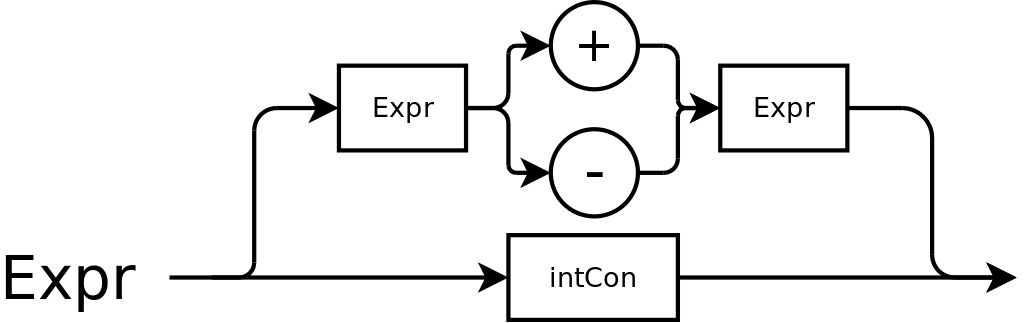
\includegraphics[width=0.6\textwidth]{./media/images/compiler/ambiguity_wrong.png}

\begin{lstlisting}[language=EBNF]
Expr = intCon | Expr ( "+" | "-" ) Expr.
\end{lstlisting}

Der Ausdruck $1-2+5$ kann mit dieser EBNF Regel auf mehreren Arten gelöst werden. Es liegt also eine Mehrdeutigkeit vor. Der Ausdruck $1-2+5$ kann dabei sowohl als $(1-2)+5$, aber auch als $1-(2+5)$ geparst werden.

\begin{tabular}{ c | c }
  $(1-2)+5=4$ & 
  $1-(2+5)=-6$ \\
  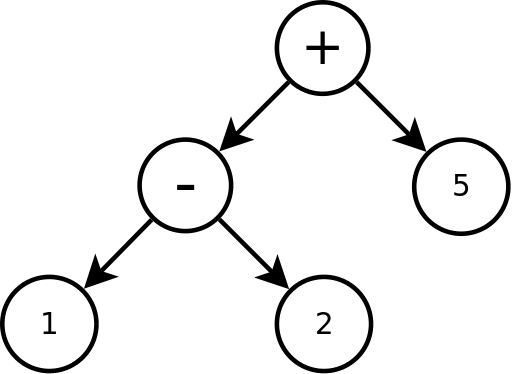
\includegraphics[width=0.2\textwidth]{./media/images/compiler/ambiguity_tree_correct.png} & 
  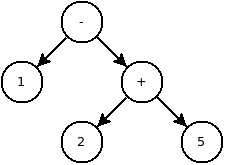
\includegraphics[width=0.2\textwidth]{./media/images/compiler/ambiguity_tree_wrong.png} \\
\end{tabular}
\subhtlParagraph{Eindeutige EBNF Regel}

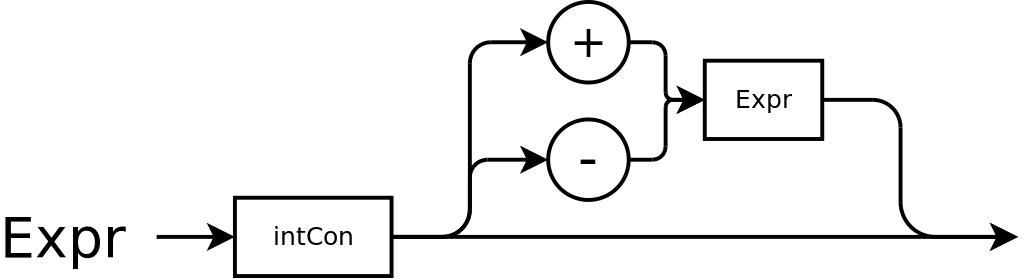
\includegraphics[width=0.6\textwidth]{./media/images/compiler/ambiguity_correct.png}

\begin{lstlisting}[language=EBNF]
Expr = intCon [ ( "+" | "-" ) Expr ].
\end{lstlisting}

Der Ausdruck $1-2+5$ kann mit dieser EBNF Regel nur mehr auf eine Art gelöst werden. Dabei werden die Operatoren links-assoziativ behandelt. Der Ausdruck $1-2+5$ wird als $(1-2)+5$ ausgewertet, was Mathematisch den korrekte Weg darstellt.

\subsubsection{EBNF-Beispiele}

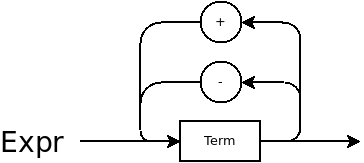
\includegraphics[width=0.5\textwidth]{./media/images/compiler/ebnf_expr.png}

\begin{lstlisting}[language=EBNF]
Expr = Term { ( "+" | "-" ) Term }.
\end{lstlisting}

Eine Expression\footnote{\url{https://de.wikipedia.org/wiki/Ausdruck_(Programmierung)}} besteht dabei aus einem Term, und dann optional wiederum aus einem ''+'' oder ''-'' gefolgt von einem weiterem Term.

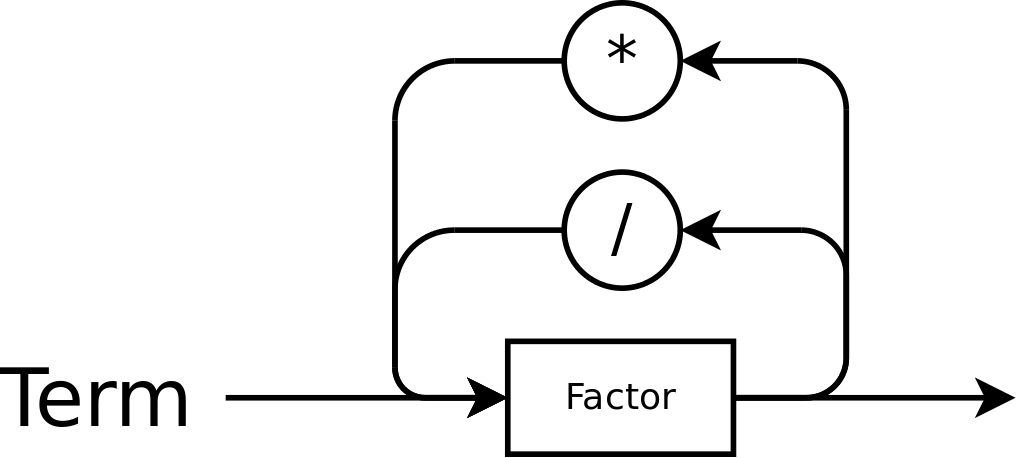
\includegraphics[width=0.5\textwidth]{./media/images/compiler/ebnf_term.png}
\begin{lstlisting}[language=EBNF]
Term = Factor { ( "*" | "/" ) Factor }.
\end{lstlisting}

Das Nichtterminalsymbol Term stellt wiederum eine Produktionsregel dar, welche aus einem Faktor, und dann optional wiederum aus einem ''*'' oder ''/'' gefolgt von einem weiterem Faktor besteht.

Durch solche einfachen Regeln können z.B.: Mathematische Regeln wie Punkt vor Strich eindeutig und korrekt in einen Syntaxbaum übersetzt werden.

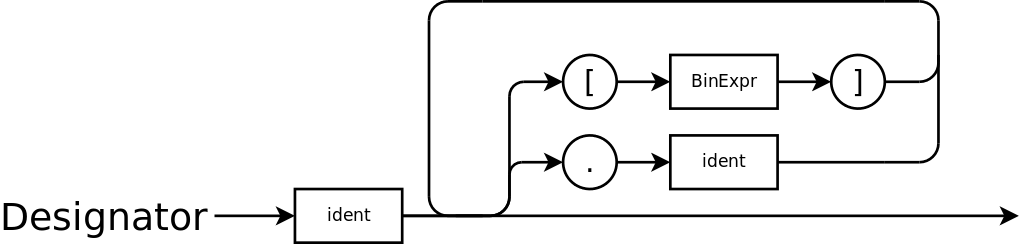
\includegraphics[width=\textwidth]{./media/images/compiler/ebnf_designator.png}
\begin{lstlisting}[language=EBNF]
Designator = ident { "." ident | "[" BinExpr "]" }.
\end{lstlisting}

%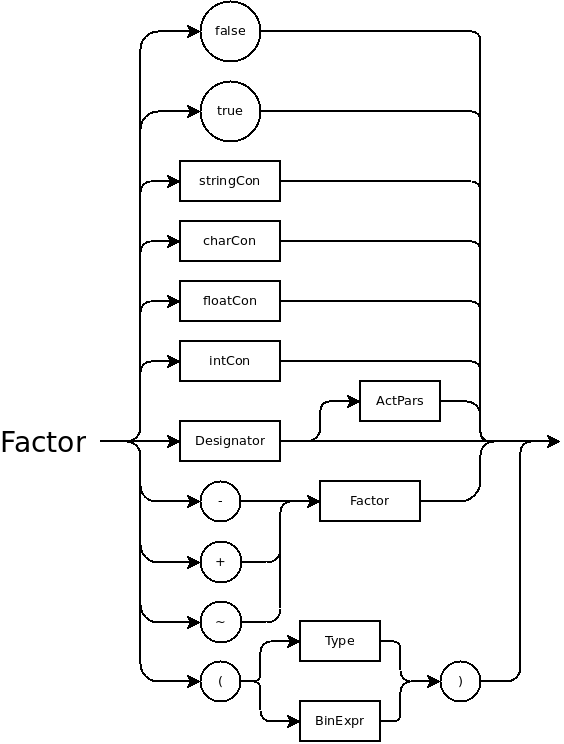
\includegraphics[width=0.6\textwidth]{./media/images/compiler/ebnf_factor.png}

\newpage

\subsection{Lexikalische Analyse - Scanner}

Bei der Lexikalischen Analyse zerlegt der sogenannt Scanner\footnote{\url{https://de.wikipedia.org/wiki/Tokenizer}} den Zeichenstrom in einen sogenannten Tokenstrom. Ein sogenannter Token\footnote{\url{https://de.wikipedia.org/wiki/Token_(\%C3\%9Cbersetzerbau)}} stellt dabei eine logische Einheit dar (z.B.: eine variable, oder ein Operatorzeichen), und wird nicht mehr weiter zerlegt (Terminalsymbol).

\htlParagraph{Zeichenstrom}

Der Scanner bekommt einen Zeichenstrom, welcher aus einzelnen Zeichen besteht. Ein Zeichen ist z.B. ein Buchstabe, eine Zahl oder Sonderzeichen wie ''='', oder ''+''.


\includegraphics[width=0.6\textwidth]{./media/images/compiler/input_characterstream.png}

\htlParagraph{Resultierender Tokenstrom}

Aus diesem Zeichenstrom werden dann die Tokens extrahiert, welche dann die sogenannten Terminalsymbole in der EBNF bzw. BNF darstellen. Tokens k\"onnen dabei aus 1. oder mehreren Zeichen bestehen.

Manche Tokens wie z.B. Variablen oder Konstanten besitzen au\ss{}er der Tokennummer desweiteren noch einen Tokenwert, mit dem sp\"ater z.B. der Variablenname, oder der Wert einer Variable ausgelesen werden kann.

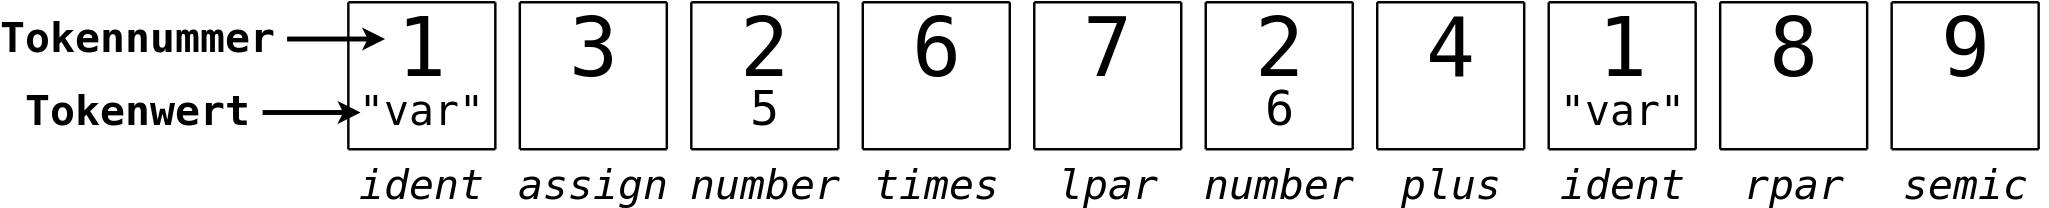
\includegraphics[width=\textwidth]{./media/images/compiler/scanner_tokenstream.png}

\subsection{Syntaxanalyse - Parser}

Der Parser\footnote{\url{https://de.wikipedia.org/wiki/Parser}} wandelt danach den Tokenstrom in einen Syntaxbaum um, welcher das Programm repräsentiert.

Es gibt verschiedene Verfahren um dies zu bewerkstelligen. Wir verwenden f\"ur unser Projekt Coco/R\footnote{\url{https://de.wikipedia.org/wiki/Coco/R}}, welcher einen LL(k)\footnote{\url{https://de.wikipedia.org/wiki/LL(k)-Grammatik}} Parser implementiert, wobei im Normalfall $k = 1$ ist. Falls $k > 1$ ist, muss f\"ur diesen Fall eine eigene Funktion implementiert werden, welche entscheidet wie der Parser weiterarbeiten soll.

Ein LL(1) Parser arbeitet dabei so, dass er jeweils um 1. Token nach vorne schaut, und mithilfe dieser Information den weiteren Parservorgang steuert.

% http://amor.cms.hu-berlin.de/~kunert/papers/lr-analyse/

\newpage

\htlParagraph{Syntaxbaum}

Der Parser \"ubersetzt den Tokenstrom in einen sogenannten Syntaxbaum\footnote{\url{https://de.wikipedia.org/wiki/Syntaxbaum}}, welcher die Struktur des Programmes repr\"asentiert.

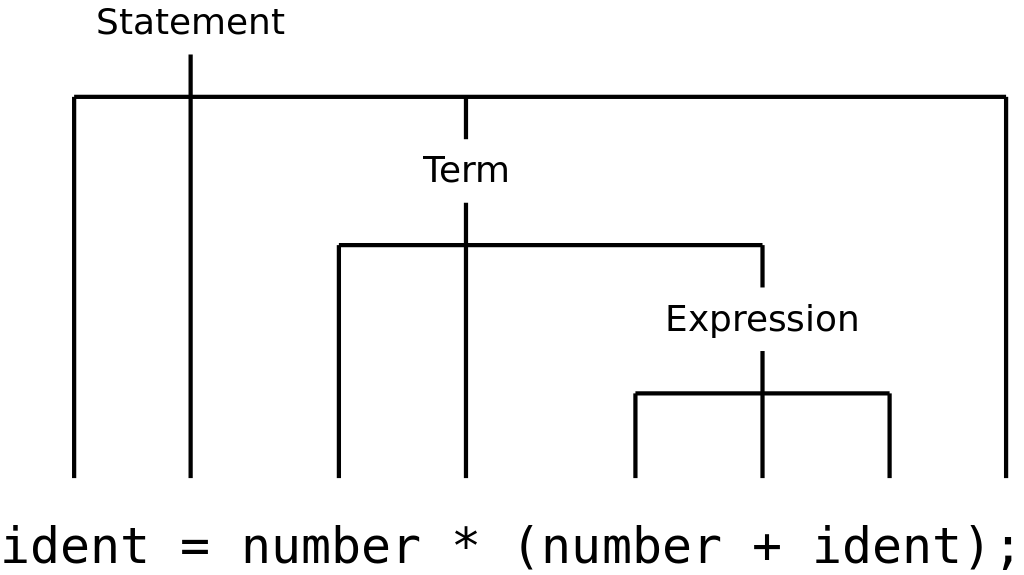
\includegraphics[width=0.6\textwidth]{./media/images/compiler/parser_syntaxtree.png}

\subsection{Abstrakter Syntaxbaum}

Der ''allgemeine'' Syntaxbaum enth\"alt viele unn\"otigen Daten, welche beim Abstraken Syntaxbaum\footnote{\url{https://de.wikipedia.org/wiki/Abstrakter_Syntaxbaum}} nicht mehr vorhanden sind. Der Abstrakte Syntaxbaum stellt somit eine Baumrepr\"asentation der wesentlichen Syntax eines Programmes dar.

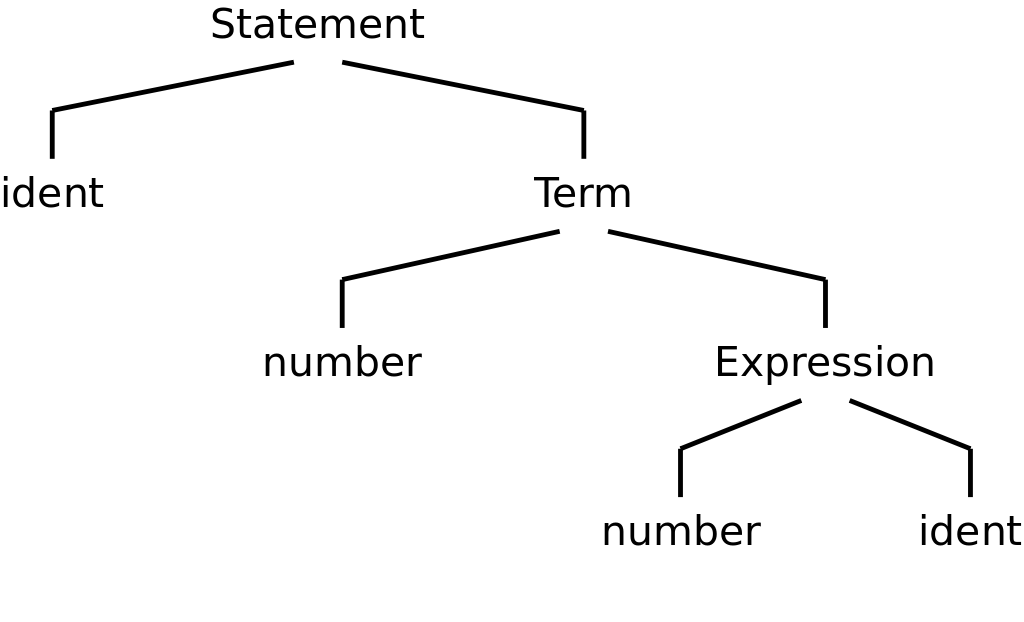
\includegraphics[width=0.6\textwidth]{./media/images/compiler/abstract_syntaxtree.png}

\subsubsection{homogene und heterogene Syntaxbäume}

Der Abstrakte Syntaxbaum kann entweder aus einheitlichen Knoten (homogen) oder aus verschiedenen Knoten (heterogen) aufgebaut sein.\footnote{\url{https://wiki.fernuni-hagen.de/eclipse/index.php/Abstract_Syntax_Tree_(AST)\#Konzept_des_Syntaxbaums}}

\subsection{Attributierte Gramatik}

%\footnote{\url{https://de.wikipedia.org/wiki/Attributgrammatik}}
Bei der Attributierten Gramatik\footnote{\url{http://steffenpingel.de/files/papers/ast.pdf}} werden Berechnungsvorschriften direkt in die Gramatik eingef\"ugt. Dadurch k\"onnen w\"arend des Parsens unter anderem Syntaxbedingungen wie z.B. Typpr\"ufungen durchgef\"uhrt werden.

In Coco/R werden diese Berechnungsvorschriften mit ''(.'' eingeleitet und mit ''.)'' beendet. Zwischen diesen Klammern befindet sich dann der Quellcode, welcher ausgef\"uhrt wird, falls der Parser den Ausdruck durchl\"auft.

\htlParagraph{Beispiel}

\begin{lstlisting}[language=EBNF]
Type<out Struct type>
= 
ident     (.  // check if a type with the given name exist
              Obj obj = tab.find(t.val);
              if(obj.kind != Obj.TYPE)
                  SemErr(obj.name + " is not a type");

              type = obj.type; .)
. 
\end{lstlisting}

In diesem Beispiel pr\"uft die Berechnungsvorschrift ob bereits ein Identifier mit dem gew\"ahlten Namen definiert wurde (passiert in der Funktion tab.find(t.val);), und ob der gefundene Identifier ein Typ ist. 

Falls eine dieser Syntaxbedingungen fehlschl\"agt, wird ein Semantischer Fehler geworfen. So werden w\"ahrend des Parsens nicht nur Syntaxfehler, sondern auch logische Fehler detektiert (z.B. fehlende Variablendeklaration).

Desweiteren kann durch diese Berechnungsvorschriften ein Abstrakter Syntaxbaum aufgebaut werden. Eine EBNF-Regel stellt nicht unbedingt einen Knoten im Abstrakten Syntaxbaum dar, da z.b. Variablendeklarationen oft in sogenannte Symboltabellen gespeichert werden.

\subsection{Symboltabelle}

Die Symboltabelle\footnote{\url{https://de.wikipedia.org/wiki/Symboltabelle}} ist eine Datenstruktur in der Variablen und Funktionsdeklarationen gespeichert werden. Sie umfasst dabei Informationen wie z.b. Zeile, in der die Variable/Funktion deklariert wurde, die gr\"o\ss{}e des Datentypes, oder auch den Wert welchen mit welchem die Variable deklariert wurde (Konstanten).

Mithilfe der Symboltabelle wird unter anderem festgestellt, ob eine Variablen deklariert wurde, oder wie viel Speicher f\"ur eine Funktion reserviert werden muss.

%, und l\"ost m\"ogliche Namensprobleme auf.\footnote{\url{https://de.wikipedia.org/wiki/Namensraum}}

\subsection{Scope}

%	--------------------------------------------------------
% 	Lösungsansätze
%	--------------------------------------------------------
%%!TEX root=../Vorlage_DA.tex
%	########################################################
% 				Lösungsansätze
%	########################################################


%	--------------------------------------------------------
% 	Lösungsansätze
%	--------------------------------------------------------
\section{Lösungsansätze}


%	--------------------------------------------------------
% 	Realisierte Lösungen
%	--------------------------------------------------------
%!TEX root=../Vorlage_DA.tex
%	########################################################
% 				Realisierte Lösungen
%	########################################################


%	--------------------------------------------------------
% 	Realisierte Lösungen
%	--------------------------------------------------------
\section{Realisierte Lösungen}

%	--------------------------------------------------------
% 	EBNF
%	--------------------------------------------------------
%!TEX root=../Vorlage_DA.tex
%	########################################################
% 				EBNF
%	########################################################

\subsection{EBNF}

\begin{lstlisting}[language=EBNF]
CMM	= { ConstDecl | StructDecl | VarDecl | ProcDecl }.
\end{lstlisting}

\begin{lstlisting}[language=EBNF]
ConstDecl = "const" Type ident "=" 
  ( ( "true" | "false" ) 
    | intCon
    | floatCon
    | charCon
    | stringCon
  ) ";".
\end{lstlisting}

%	--------------------------------------------------------
% 	Lexikalische Struktur
%	--------------------------------------------------------
%!TEX root=../Vorlage_DA.tex
%	########################################################
% 				Lexikalische Struktur
%	########################################################

\subsection{Lexikalische Struktur}


%	--------------------------------------------------------
% 	Syntaxbäume
%	--------------------------------------------------------
%!TEX root=../Vorlage_DA.tex
%	########################################################
% 				Lexikalische Struktur
%	########################################################

\subsection{Syntaxbäume}


%	--------------------------------------------------------
% 	Standardbibliotek
%	--------------------------------------------------------
%!TEX root=../Vorlage_DA.tex
%	########################################################
% 				Lexikalische Struktur
%	########################################################

\subsection{Standardbibliotek}

Der C-Compact Standard besitzt zur Kommunikation zwischen Programm und Oberfläche nur wenige Funktionen. Funktionalitäten wie Ein/Ausgabe von Strings, das Umwandeln von int nach string,... müssen daher direkt in C-Compact implementiert werden.

In C-Compact sind die wichtigsten Funktionen, welche in der C-Standardbibliotek vorkommen nachimplementiert.

\subsection{Kontextbedingungen}

\subsection{Typkonvertierung}

\subsection{Scope}

\subsection{Strings}

%	--------------------------------------------------------
% 	Sprachspezifikation
%	--------------------------------------------------------
%!TEX root=../Vorlage_DA.tex
%	########################################################
% 				Allgemeiner Teil (Theorie)
%	########################################################


%	--------------------------------------------------------
% 	Sprachspezifikation
%	--------------------------------------------------------
\newpage
\section{Sprachspezifikation}

\subsection{Pr\"aprozessor}

Unser Pr\"aprozessor erm\"oglicht die Nutzung mehrer Dateien und verf\"ugt \"uber die Funktion einzelne Codeteile zu deaktivieren, wie es auch in C der Fall ist. Pr\"aprozessorargumente beginnen dabei jeweils mit einem Hashtag, gefolgt von der jeweiligen Direktive und einem oder mehreren Argumenten.

\subsubsection{\#include Direktive}

Mithilfe eines \#include k\"onnen andere Dateien eingebunden werden. Es gibt dabei 2. Arten von \#include, welche sich durch den jeweiligen Suchpfad unterscheiden. Aus Technischer Sicht kopiert der Pr\"aprozessor die jeweilige Datei an die Stelle wo das \#include geschrieben ist.

\htlParagraph{Suche im Standard-Include-Pfad}

Der Standard-Include-Pfad stellt der Ordner clib dar, in welchem sich die Standardbibliothek befindet.

\begin{lstlisting}[language=C]
#include <stdio.h>
\end{lstlisting}

\htlParagraph{Suche im aktuellen Verzeichnis}

Wenn selbst geschriebene Programmdateien eingebunden werden sollen wird der Pfad relativ zum aktuellen Verzeichnis angegeben. So ist es m\"oglich gro\"o\ss{}ere Projekte auf Basis mehrere Dateien zu entwickeln.

\begin{lstlisting}[language=C]
#include "foo.cmm"
\end{lstlisting}

\subsubsection{\#define Direktive}

Es ist m\"oglich den w\"ahrend des Pr\"aprozessorvorganges Variablen zu definieren, welche aber nur im Pr\"aprozessor ausgewertet werden k\"onnen. Es ist nicht m\"oglich mithilfe eines \#define Quelltext zu ver\"andern, wie es in C m\"oglich ist!

Es ist m\"oglich einem Define einen Wert zuzuweisen, welcher eine Ganze Zahl sein muss. Falls kein Wert angegeben ist wird 1 angenommen.

\begin{lstlisting}[language=C]
#define __DEFINE_WITHOUT_VALUE__
#define __DEFINE_WITH_VALUE__ 0
\end{lstlisting}

Falls ein \#define mit dem gleichen Namen bereits existiert, wird dieses \"uberschrieben.

\subsubsection{\#undef Direktive}

Mithilfe eines \#undef kann eine definierte Variable gel\"oscht werden. Die Variable steht somit nicht mehr zur verf\"ugung, bis die Variable erneut definiert wird.

\begin{lstlisting}[language=C]
#undef __DEFINE_WHICH_IS_NOW_DELETED__
\end{lstlisting}

\subsubsection{\#ifdef, \#ifndef, \#else und \#endif Direktive}

Es ist m\"oglich abzufragen ob es eine bestimmte Variablendefinition gibt, oder nicht gibt. Diese Abfrage wird mit den Pr\"aprozessorargumenten \#ifdef bzw. \#ifndef eingeleitet, und muss mit einem \#endif enden. Falls es notwendig ist auch f\"ur das Gegenargument code auszuf\"uhren kann dies mithilfe eines \#else eingeleitet werden.

Eine Variable gilt als definiert wenn sie mithilfe eines \#define erzeugt wurde, und einen Wert ungleich 0 besitzt.

\begin{lstlisting}[language=C]
#ifdef __SOME_DEFINE__
	// ... Do something if __SOME_DEFINE__ is defined
#else
	// ... Do something if __SOME_DEFINE__ is not defined
#endif
\end{lstlisting}

\subsubsection{Beispiel}

Der Pr\"aprozessor wird besonders daf\"ur ben\"otigt, dass Bibliotheken bei mehrfachen \#include keine Fehler verursachen. Dazu ist es notwendig dass die Bibliothek bei mehrfachen \#include die nachfolgenden Ignoriert. Dies stellt ein Standardkonstrukt in der C Programmierung dar.

\begin{lstlisting}[language=C]
#ifndef __CLIB_EXAMPLE__

	#define __CLIB_EXAMPLE__
	
	// ... some includes if required
	#include <stdio.h>

	// ... here is the executed code of the file

#endif /* __CLIB_EXAMPLE__ */
\end{lstlisting}

Zuerst wird ermittelt, ob die Bibliothek bereits eingebunden wurde (falls dies der Fall ist, ist die jeweilige Variable definiert), und \#ifndef ignoriert infolge den folgenden Code bis zum \#endif.

Falls der Code aber das erste mal eingebunden wurde, ist die Variable (in diesem Beispiel $\_\_CLIB\_EXAMPLE\_\_$) noch nicht definiert worden. Folglich wird der Code welcher sich in \#ifndef befindet ausgef\"uhrt, wo unter anderem die jeweilige Variable definiert wird, welche einzigartig f\"ur die jeweilige Bibliothek sein muss.

\subsection{Kommentare}

Bereiche welche als Kommentar\footnote{\url{https://de.wikipedia.org/wiki/Kommentar_(Programmierung)}} deklariert sind, werden vom Pr\"aprozessor und vom Compiler ignoriert. Es gibt dabei 2. Arten von Kommentare.

\htlParagraph{Zeilenkommentar}

Ein Zeilenkommentar beginnt mit einem //, und endet mit dem Ende der Zeile.

\begin{lstlisting}[language=C]
// this is a simple line comment
\end{lstlisting}

\htlParagraph{Blockkommentar}

Ein Blockkommentar beginnt mit einem /* und enden bei dem ersten auftreten eines */.

\begin{lstlisting}[language=C]
/* this is a
   blockcomment */
\end{lstlisting}

\subsection{Datentypen}

Der gew\"ahlte Datentyp\footnote{\url{https://de.wikipedia.org/wiki/Datentyp}} gibt an welche Art von Daten gespeichert werden k\"onnen. Es gibt primitive Datentypen, welche gro\"ss{}teils auch Arithmetische Datenoperationen unterst\"utzen, und Zusammengesetzte Datentypen welche aus einem oder mehreren primitiven Datentypen aufgebaut sind.

\subsubsection{Primitive Datentypen}

\htlParagraph{void}

void bezeichnet keinen eigentlichen Typen, und ist nur f\"ur die Definition von Funktionen erlaubt, welche nichts zur\"uckgeben.

\begin{lstlisting}[language=C]
void foo() {
}
\end{lstlisting}

\htlParagraph{bool}

bool unterst\"utzt die beiden Wahrheitswerte true und false. Wenn ein int als bool ausgewertet wird, stellt 0 false dar, und ungleich 0 ist true.

\begin{lstlisting}[language=CMM]
bool b;

bool foo() {
	return true;
}
\end{lstlisting}

\htlParagraph{char}

Ein char stellt ein einzelnes alphanumerisches Zeichen, ein Leerzeichen oder das Sonderzeichen \textbackslash{}r, \textbackslash{}n, \textbackslash{}t, \textbackslash{}0, \textbackslash{}' oder \textbackslash{}\textbackslash{} dar.

\begin{lstlisting}[language=CMM]
char ch;

char foo() {
	return 'c';
}
\end{lstlisting}

\htlParagraph{int}

Ein int stellt eine ganzzahlige Zahl dar, welche einen Wert zwischen $-2147483648$ und $2147483647$ haben muss.

\begin{lstlisting}[language=CMM]
int i;

int foo() {
	return 1234;
}
\end{lstlisting}

\htlParagraph{float}

\begin{lstlisting}[language=CMM]
float f;

float foo() {
	return 1.2;
}
\end{lstlisting}

\htlParagraph{string}

\begin{lstlisting}[language=CMM]
string s;

string foo() {
	return "Hello World";
}
\end{lstlisting}

\subsubsection{Konstanten}

Konstanten sind Variablen, welche nicht ver\"andert werden k\"onnen. Der Wert muss dabei bei der Deklaration angegeben werden, und muss dem Datentyp der Konstante entsprechen (Typumwandlungen sind nicht zul\"assig!).

\begin{lstlisting}[language=CMM]
const int i = 1234;
\end{lstlisting}

\subsubsection{Strukturen}

Strukturen sind zusammengesetzte Datentypen welche aus 1. oder mehreren Datentypen bestehen. Eine definierte Struktur stellt einen neuer Datentyp dar, von welchem Variablen definiert werden k\"onnen, welche man auch an Funktionen \"ubergeben kann.

Strukturen k\"onnen nicht auf sich selbst verweisen, da es ansonsten eine endlosen Rekursion darstellen w\"urde. Des weiteren k\"onnen keine Werte bei der Definition einer Struktur angegeben werden.

\begin{lstlisting}[language=CMM]
struct Point {
    int x, y;
    string name;
}

Point p;
\end{lstlisting}

\subsubsection{Arrays}

Arrays sind Felder von Datentypen, wobei ein einzelnes Feld mithilfe eines sogenannten Index spezifiziert werden kann.

Falls ein Array in einer Funktion definiert wird, kann diesem ein Initialisierungswert zugewiesen werden, welcher das Array mit definierten Werten f\"ullt.

\begin{lstlisting}[language=CMM]
char cArr[10];
int arr[5][5];
\end{lstlisting}

\subsubsection{Typumwandlung}

Es ist m\"oglich Datentypen in einen anderen Umzuwandeln. Dies kann einerseits implizit geschehen, oder muss explizit angegeben werden. Es ist nicht m\"oglich jeden Datentyp in jeden anderen umzuwandeln. Strukturen und Arrays können bis auf besondere ausnahmef\"alle nicht umgewandelt werden.

\htlParagraph{Implizite Typumwandlung}

Bei der Impliziten Typumwandlung wird diese automatisch w\"ahrend des Compiliervorganges durchgef\"urt.

\begin{lstlisting}[language=CMM]
float f = 1 + 2.5; // 1 is implicit converted to float
\end{lstlisting}

\htlParagraph{Explizite Typumwandlung}

Die explizite Typumwandlung ist besonders dann notwendig, falls ein Datentyp in einen anderen umgewandelt werden muss, welcher weniger Daten speichern kann als sein Ursprungstyp.

\begin{lstlisting}[language=CMM]
char ch = (char)48; // explicite conversation of int to char
\end{lstlisting}

\subsection{Funktionen}

Funktionen k\"onnen maximal 1. R\"uckgabewert besitzen, und beliebig viele Argumente. Es ist m\"oglich Referenzen auf Variablen zu \"ubergeben, wobei dies bei Arrays immer der Fall ist.

Zus\"atzlich ist es m\"oglich die Funktion mit dem Schl\"usselwort library in eine Bibliotheksfunktion umzuwandeln, welche vom Debugger immer \"ubersprungen wird.

\begin{lstlisting}[language=CMM]
int library foo(int a, int b[], int &c) {
	c = 3;
	return b[3];
}
\end{lstlisting}

\subsubsection{Vorw\"artsdeklarationen}

Vorw\"artsdeklarationen werden ben\"otigt wenn auf eine Funktion zugegriffen werden muss, bevor diese vollst\"andig inklusive interner Logik Deklariert wurde. Dabei wird die Funktionsdeklaration kopiert, und anstatt mit geschwungenen Klammern und der Funktionslogik, nur mit einem Strichpunkt abgeschlossen.

\begin{lstlisting}[language=CMM]
int foo(int a);

int foo(int a) {
	if(a == 0)
		return 0;
	return (a + foo(a-1));
}
\end{lstlisting}

\subsubsection{Vorimplementierte Funktionen}

Es gibt eine gewisse Funktionen welche bereits im Interpreter und Compiler implementiert sind, um C-Compact eine Interaktion mit dem Debugger zu erm\"oglichen.

\htlParagraph{print}

Schreibt 1. Zeichen in die Ausgabe. 

\begin{lstlisting}[language=CMM]
print('a');
\end{lstlisting}

\htlParagraph{read}

Lese das n\"achste Zeichen vom Eingabestrom.

\begin{lstlisting}[language=CMM]
char c = read();
\end{lstlisting}

\htlParagraph{printf}

Schreibe eine Formatierte Ausgabe in die Ausgabe. Diese Funktion unterst\"utzt beliebig viele Argumente, wobei f\"ur jede Platzhalter im String ein Argument angegeben werden muss.

\begin{lstlisting}[language=CMM]
printf('a= %d, b=%f\n', 10, 2.2);
\end{lstlisting}

\subhtlParagraph{Platzhalter}

Ein Platzhalter definiert ein Variable welche in einem spezifizierten Ausgabeformat ausgegeben wird. 

 \begin{tabular}{l | l}
  Typ & Platzhalter \\
  \hline
  char & \%c \\
  int & \%d \\
  hex & \%x \\
  float & \%f \\
 \end{tabular}

\htlParagraph{length}

Mithilfe der length-Funktion ist es m\"oglich die L\"ange eines Strings zu ermitteln.

\begin{lstlisting}[language=CMM]
int l = length("Hello World");
\end{lstlisting}

\htlParagraph{time}

Diese Funktion gibt die vergangenen Sekunden aus beginnend mit dem 1. Januar 1970. Diese Funktion wird unter anderem f\"ur den Zufallsgenerator ben\"otigt.

\begin{lstlisting}[language=CMM]
int timestamp = time();
\end{lstlisting}

\htlParagraph{\_\_is\_def\_***\_\_}

Dies is ist eine interne Funktion, welche f\"ur die Bibliothek ben\"otigt wird, und zugriff auf den Speicher gibt. Es gibt dabei f\"ur jeden Datentyp eine eigene Funktion, welche true zur\"uckliefert wenn die Variable bereits initialisiert wurde. Ansonsten wird false zur\"uckgegeben.

\begin{lstlisting}[language=CMM]
bool test;
bool isTestInitialized = __is_def_bool__(test);
\end{lstlisting}

\htlParagraph{\_\_assert\_\_}

Wenn der erste Parameter false ist, wird der Interpreter angehalten und eine definierte Fehlermeldung ausgegeben. diese Funktion wird auch nur in Bibliotheksfunktionen verwendet, um unter anderem Eingabedaten auf Grenzwerte und Valid\"at zu zu pr\"ufen.

\begin{lstlisting}[language=CMM]
__assert__(false, "some error occured");
\end{lstlisting}

\subsection{Operatoren}

C-Compact unterst\"utzt alle Standardoperatoren wie Plus, Minus, aber auch Stiftoperatoren und binäre Operatoren. Zu beachten ist dass Logische Operatoren nur in Bedingungen genutzt werden k\"onnen, nicht aber in normalen Ausdr\"ucken. Es gilt Punkt vor Strich vor Shift vor bin\"are Operatoren. Diese Reihenfolge kann nat\"urlich mit Klammern ver\"andert werden.

\begin{lstlisting}[language=CMM]
 a = ((5 + 2 - 3) / 4) << 2; // a = 4
 b = 0x000f & 0x1003; // b = 0x0003
\end{lstlisting}

\subsubsection{Punktoperatoren}

\subsubsection{Strichoperatoren}

\subsubsection{Shiftoperatoren}

Der Logische Shiftoperator\footnote{\url{https://de.wikipedia.org/wiki/Logische_Verschiebung}} verschieben den Inhalt einer Speicherzelle logisch um eine gew\"ahlte L\"ange. Zu beachten ist dass Daten welche außerhalb der Speicherzelle geschrieben werden gel\"oscht werden, und ansonsten undefinierte Bits mit 0 initialisiert werden.

\begin{figure}[h]
\centering
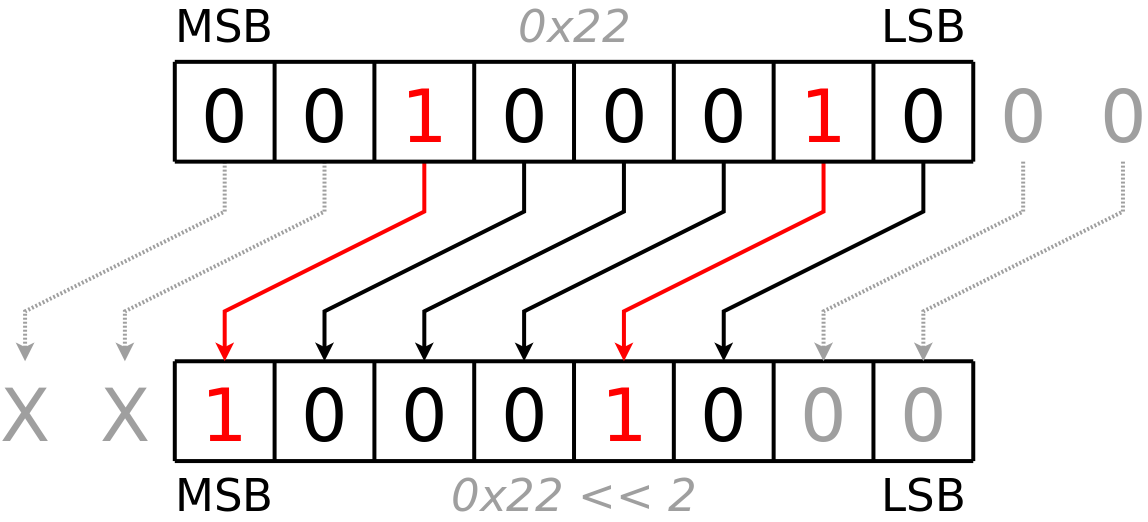
\includegraphics[width=0.8\textwidth]{./media/images/compiler/language_specification_shift_operator.png}
\caption{Bitweise Verschiebung einer 1.Byte Variable um 2 nach links}
\label{language_specification_shift_operator}
\end{figure}

\subsubsection{Bin\"are Operatoren}

Bin\"are Operatoren f\"uhren jede Operation einzeln pro Bit aus, ohne Nachtbarbits zu ber\"ucksichtigen.

\begin{figure}[h]
\centering
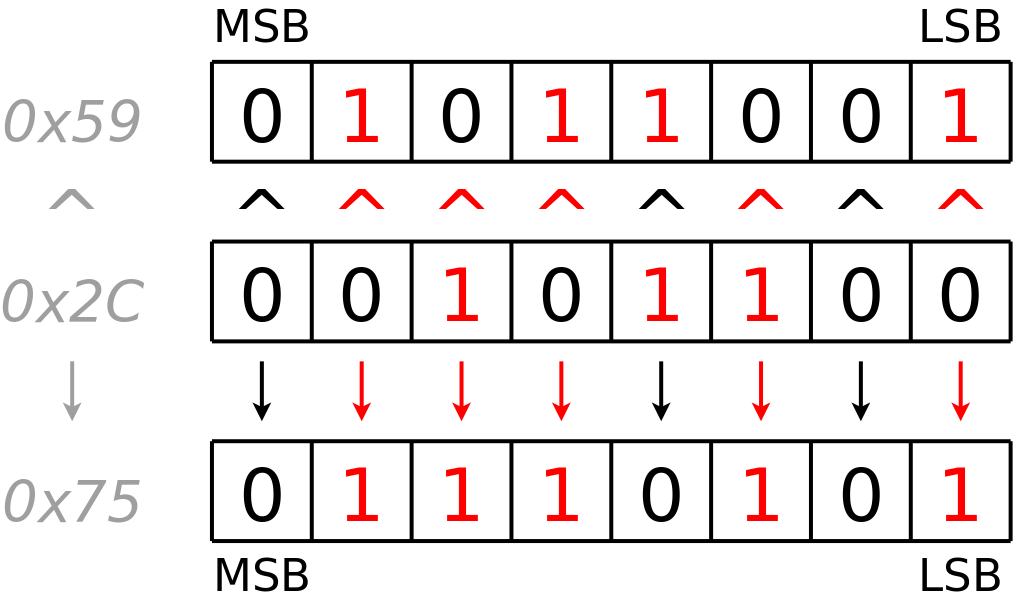
\includegraphics[width=0.7\textwidth]{./media/images/compiler/language_specification_binary_operator_xor.png}
\caption{Bitweises XOR von 2. Variablen}
\label{language_specification_binary_operator_xor}
\end{figure}


%	--------------------------------------------------------
% 	Kalkulation
%	--------------------------------------------------------
%\section{Kalkulation}

%	--------------------------------------------------------
% 	Arbeitseinteilung
%	--------------------------------------------------------
%\section{Arbeitseinteilung}

%	--------------------------------------------------------
% 	Interpreter
%	--------------------------------------------------------	
%!TEX root=../Vorlage_DA.tex
%	########################################################
% 				Projektbeschreibung
%	########################################################


%	--------------------------------------------------------
% 	Überschrift, Inhaltsverzeichnis
%	--------------------------------------------------------
\chapter{Interpreter}


%	--------------------------------------------------------
% 	Allgmeine Hinweise
%	--------------------------------------------------------
\section{Allgemeiner Teil (Theorie)}

\subsection{Aufbaumöglichkeiten eines Interpreters}

\subsubsection{Bytecode Interpreter}
Bei der Compilierung wird eine Zwischensprache erzeugt, welche aus einer Sammlung von Befehlen besteht. Dadurch wird das System
betriebssystemunabhängig und der Code ist nahezu hardwareunabhängig.

Jedoch muss zum Ausführen des Programmes, welches in die Zwischensprache übersetzt wurde, eine virtuelle Maschine vorhanden sein.
Dadurch, dass während der Ausführung des Programmes compiliert werden muss, sinkt die Geschwindigkeit gegenüber
nativ compilierten Programmen.

%Durch die Verwendung des Just-in-time-compilation Verfahrens kann die Geschwindigkeit wieder verbessert werden.

\subsubsection{Abstrakter Syntaxbaum Interpreter}
Bei dem von uns gewählten Ansatz wird der Quellcode in einen optimierten abstrakten Syntaxbaum übersetzt. Dieser Baum wird während der Laufzeit
abgearbeitet. Jeder Knoten muss nur einmal durchsucht werden. Im Vergleich zu einem Bytecode wird beim Abstrakten Syntaxbaum die Struktur
des Programmes beibehalten. Dadurch kann man Fehler im Programm leichter analysieren.

%\subsubsection{Just-in-time compilation}
%Um Plattformunabhängigkeit gewährleisten zu können, ist es notwendig, gewisse Teile während der Laufzeit zu kompilieren. 
%Darunter leidet aber die Ausführungsgeschwindigkeit. Deshalb wurde ein Verfahren entwickelt, welches versucht,
%diesen Nachteil zu lindern.

%Während der Anwendung des Programmes wird ein lauffähiger Maschinencode erzeugt. Es werden hierbei oft verwendete Programmteile
%während der Laufzeit kompiliert und für einen späteren Gebrauch zwischengespeichert. Hierbei ist es wichtig, dass die Compilation nicht
%zu aufwendig ist, da sonst die Geschwindigkeit des Programmes darunter leiden könnte.

\subsection{Call Stack}
Der sogenannte Call Stack, auch Aufrufstapel genannt, enthält während der Laufzeit Informationen über die gerade ablaufenden 
Unterprogramme. 

%Der Call Stack wird mit einem Befehlssatz zum Befüllen, Abbauen und zum Wiedereintritt in ein anderes Unterprogramm bearbeitet.

Sobald mehrere Threads oder Prozesse ausgeführt werden sollen, muss für jeden gewünschten Prozess ein eigener Call Stack eingerichtet
werden, damit sich die Variablen und Rücksprungadressen nicht überschreiben.

\subsubsection{Lokale Variablen}
Wenn lokale Variablen verwendet werden, wird am Call Stack der nötige Variablenspeicher reserviert. Da jeder Aufruf seine
eigenen Variablen hat, sind rekursive Unterprogrammaufrufe möglich. Um vom aktuellen Aufruf auf den letzten zurückzukommen, ist
es notwendig, eine Referenzadresse auf den letzten Aufruf zu speichern.


%	--------------------------------------------------------
% 	Lösungsansätze
%	--------------------------------------------------------
%\section{Lösungsansätze}
%	--------------------------------------------------------
% 	Realisierte Lösungen
%	--------------------------------------------------------
\section{Realisierte Lösungen}
Hier wird der Aufbau des Interpreters näher erläutert und die einzelnen Funktionen werden näher vorgestellt.

Der Interpreter wurde genauso wie die anderen Komponenten in Java implementiert.
Am meisten wurde beim Aufbau des Interpreters auf die Schnittstelle zum GUI geachtet, da der Interpreter für eine einfachere
Programmdarstellung optimiert werden sollte.

Der Aufbau des Abstrakten Syntaxbaumes ist im Kapitel Compiler zu finden. Dort werden die einzeln verwendeten 
Knoten näher erläutert.

\subsection{Memory}
Ein wesentlicher Teil des Speichermodells ist die Aufbewahrung unterschiedlichster Variablen. Hierbei wird zwischen Variablen in Unterprogrammen und globalen Variablen unterschieden. \\
Für globale Variablen wird extra ein Platz reserviert. Lokale Variablen werden in einem gewissen Frame immer wieder auf und abgebaut. \\
Somit bleiben globale Variablen immer enthalten, wobei Lokale Variablen nach dem Unterprogrammaufruf erstellt werden. Sobald das Unterpgramm fertig durchlaufen ist, wird der Speicherplatz der lokalen Variablen wieder freigegeben.

\subsubsection{Aufbau unseres Stack Frames}
\begin{figure}[Stack Frame]
\begin{center}
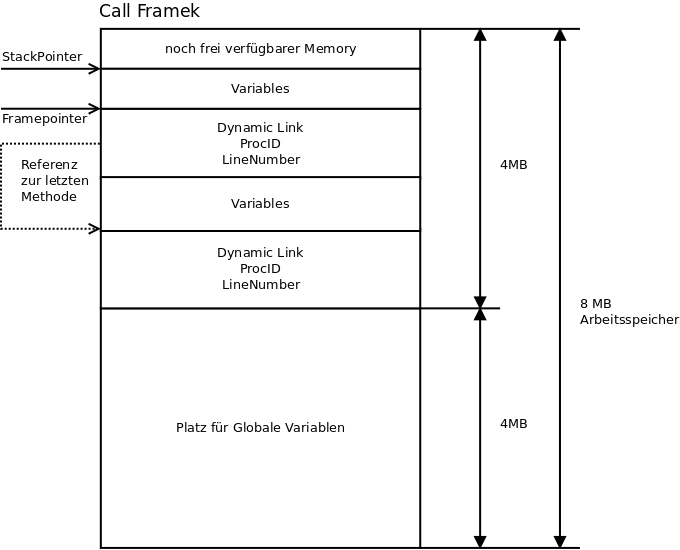
\includegraphics[width=0.9\textwidth]{./media/images/interpreter/memory/stackframe.png}
\label{stackframe1} 
\caption{Aufbau des von uns verwendeten Stack Frames}
\end{center}
\end{figure}
%--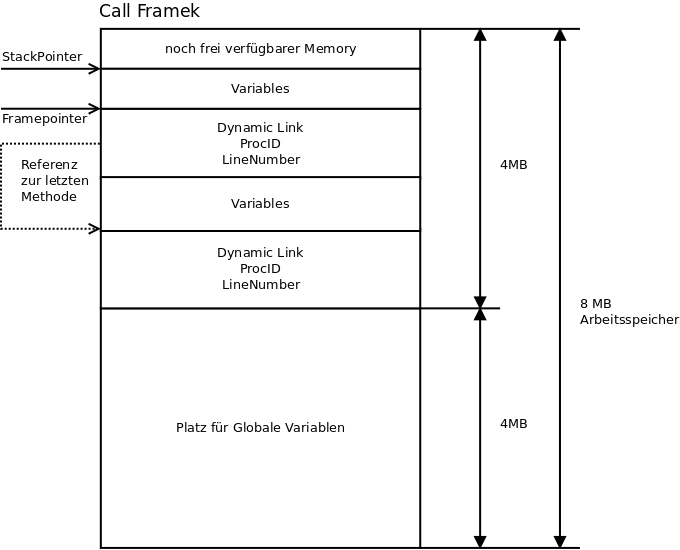
\includegraphics[scale=0.3]{./media/images/interpreter/memory/stackframe.png}

\subsection{Aufbau des Memorys}
Da für kleine Programmieraufgaben, welche man zum Erlernen einer Programmiersprache, nicht viel Arbeitsspeicher benötigt wird, sowie keine Graphische Programmierung in C Compact vorgesehen ist, haben wir uns entschieden 8 MB Arbeitsspeicher für den Memory zu reservieren.
Wie man in \ref{stackframe1} erkennen kann, wurde dieser in 2 Hälften geteilt. Davon wird der untere Teil für Globale Variablen und der obere Teil für die Unterprogramme verwendet.

\subsection{Speicherinhalte eines Unterprogramms}
Ein Unterprogramm muss grundsätzlich im Call Frame schon im vorhinein einige Variablen enthalten, welche das zurückspringen auf das letzte Unterprogramm ermöglichen. Hierfür ist der Dynamic Link zuständig. Weiters wird die LineNumber gespeichert, diese wird vom GUI benötigt, damit dieser das Programm schrittweise abarbeiten kann. Weiters ist eine ProcID vorhanden, diese ist für den Namen des Unterprogramms zuständig.

\subsubsection{Aufruf einer neuen Methode}
\begin{enumerate}
 \item Die Zeilennummer wird in den Speicher geschrieben (Größe von 4 Byte)
 \item Der Methodenname wird im Speicher vermerkt (Größe von 4 Byte)
 \item Eine Referenz des Framepointers, mit welcher man zum letzten Methodenaufruf zurückgelangen kann, wird im Speicer notiert (Größe von 4 Byte)
 \item Nun wird der Framepointer auf\footnote{Untere Referenzadresse im Memory} denselben Wert wie der Stackpointer{Obere Referenzadresse im Memory} gesetzt.
 \item Um genügend Speicher für Variablen gewährleisten zu können, muss nun zum StackPointer die vom Compiler vorgegebene Variablengröße
 hinzugefügt werden. Dort werden dann alle lokalen Variablen zwischengespeichert.
\end{enumerate}
 
\subsubsection{Schließen einer Methode}
\begin{enumerate}
 \item Der Stackpointer wird auf Framepointer gesetzt (Variablen werden entfernt).
 \item Um an den Startwert der Referenz zu gelangen müssen nun vom Stackpointer 4 Bytes abgezogen werden.
 \item Die Referenz verweißt auf den im letzten Methodenaufruf verwendeten Framepointer. Somit wird der Framepointer nun mit dem Wert
 der Referenz versehen.
 \item Um den richtigen Stackpointer zu bekommen, ist es nun notwendig den Stackpointer um den vorherigen Methodennamen und um die vorher verwendete Zeilennummer zu veringern.
 Somit muss der Stackpointer um 8 Byte veringert werden.
\end{enumerate}

\subsubsection{Speicherverwaltung}
Da bei der Speicherverwaltung viele Fehler auftreten könnten, ist es wichtig, dass diese mit verschiedensten Exceptions abgefangen werden.

Alle vom Interpreter benötigten Funktionen, sind in der statischen Klasse Memory zu finden. 

Vom Memory werden verschiedenste Datentypen unterstützt.
\begin{itemize}
 \item int - 4 Byte
 \item float - 4 Byte
 \item char - 2 Byte 
 \item boolean - 1Byte
 \item string - 4 Byte - beinhaltet jedoch nur die Adresse wo der String zu finden ist.
\end{itemize}
Alle Variablen können mit der nötigen Adresse und der zum Variablennamen passenden Funktion abgefragt werden.

Bei der Speicherung einer Variable ist die Größe der Variablen bereits bekannt, und muss nicht extra vom Interpreter herausgefunden werden. Somit muss der Interpreter nur zwischen den verschiedenen Datentypen unterscheiden und durch Aufruf der richtigen Methoden im Memory auf die richtige Adresse schreiben.

\subsection{Interpreter}
Weil wir eine einfache Darstellung der aktuellen Variablen bezweckten und den Ablauf des Programmes nicht verändern wollten, kam für 
uns nur der Abstrakte Syntaxbaum-Interpreter in Frage.

Es wurden einige Vorgaben gemacht, um ein Zusammenarbeiten zwischen Compiler und Interpreter möglich zu machen. Somit wurde eine gewisse
Baumstruktur vorgegeben. In diesem konnten die Knoten nur in einer bestimmten Reihenfolge auftreten.

\subsection{Statements}
\subsubsection{assign}
Bei einem Assign wird eine bestimmte Variable in den Memory geschrieben. Bevor dies jedoch geschehen kann, ist es notwendig,
den Datentyp herauszufinden. Dafür wird der Typ des rechten Knotens geprüft.

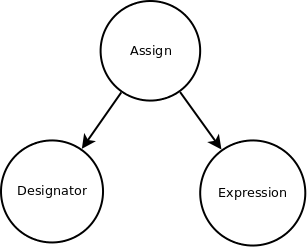
\includegraphics[width=0.4\textwidth]{./media/images/interpreter/syntaxbaum/statements/assign.png}

\subsubsection{startsequenz}
Mithilfe der Startsequenz wird das derzeitige Unterprogramm abgearbeitet.

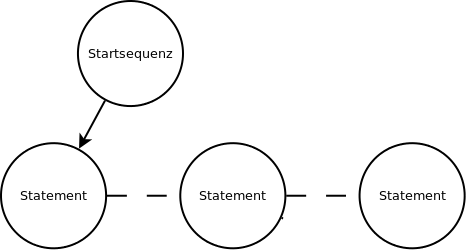
\includegraphics[width=0.6\textwidth]{./media/images/interpreter/syntaxbaum/statements/startsequenz.png}

\subsubsection{trap}
Die Trap wird dazu benötigt, um einen Unterprogrammaufruf, welcher keine Rückgabeparameter besitzt, zu beenden.

\subsubsection{if}
Auf der linken Seite des Knotens stehen die Bedingungen, auf der rechten Seite steht das auszuführende Programm, wenn die Bedingung
true ergibt.

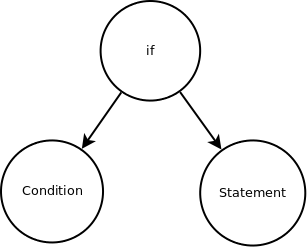
\includegraphics[width=0.4\textwidth]{./media/images/interpreter/syntaxbaum/statements/if.png}

\subsubsection{Ifelse}
Das Ifelse ist grundsätzlich genauso aufgebaut wie das If. Der wesentliche Unterschied besteht darin, dass, sobald die Condition
false ergibt, die andere if-Funktion abgearbeitet wird.

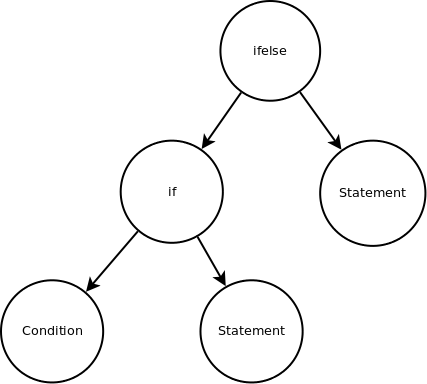
\includegraphics[width=0.4\textwidth]{./media/images/interpreter/syntaxbaum/statements/ifelse.png}

\subsubsection{while}
Sie funktioniert ähnlich wie ein If, das Statement jedoch wird so oft wiederholt, bis die Condition false ergibt.

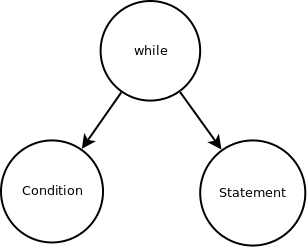
\includegraphics[width=0.4\textwidth]{./media/images/interpreter/syntaxbaum/statements/while.png}

\subsection{call}
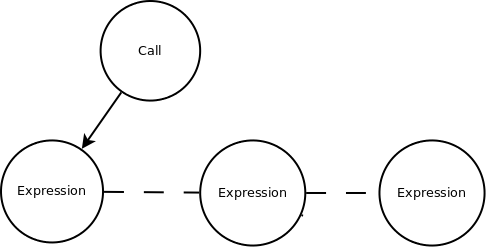
\includegraphics[width=0.6\textwidth]{./media/images/interpreter/syntaxbaum/statements/call.png}

Ein Call Knoten hat mehrere Funktionen. Die Richtige wird anhand des Namens herausgefunden. Dies sind schon vordefinierte
Funktionsnamen, welche in einem Programm nicht erneut verwendet werden können.

Hier eine Auflistung dieser Funktionen:

\subsubsection{print}
Hiermit wird ein Char-Zeichen dem StdInOut Interface übergeben. Somit kann dieses danach vom GUI ausgeben werden.

\subsubsection{read}
Wenn Read aufgerufen wird, werden vom Interface StdInOut Char-Variablen eingelesen und diese als Return Wert gesetzt und kann somit zur Weiterverarbeitung verwendet werden.

\subsubsection{length}
Hier kann man die Länge eines Strings bestimmen lassen, dieser wird wiederum als Return-Wert gesetzt.

\subsubsection{time}
``time'' dient zum Bestimmen der Zeit, welche wiederum als Return-Wert zurückgegeben wird. Wird für den implementierten Zufallsgenerator bei der Initialisierung benötigt.

\subsubsection{Normaler Aufruf}
%TODO Neu programmiert
Sobald ein Aufruf erfolgt, werden alle Variablen, welche übergeben werden sollen, in einem Objekt zwischengespeichert. Nun kann ein
neues Memoryframe geöffnet werden. Die Variablen, welche in einem Objekt zwischengespeichert wurden, können nun in das neue
Memoryframe übertragen werden.

Nun wird eine Startsequenz ausgeführt, damit der Unterprogrammaufruf abgearbeitet werden kann.

\subsection{Designators}
Auf Designators werden bestimmte Werte gespeichert. Diese können zum Beispiel normale Variablen, Arrays oder Strukturen sein. Hier ist die richtige Zuweisung der Adresse wichtig.

Designators werden in 3 Grundtypen unterschieden:
\subsubsection{Identifer}
Ein Identifer ist eine normale einfache Variable. Wenn ein Identifer aufgerufen wird, werden verschiedene Faktoren geprüft.
\begin{itemize}
 \item Falls diser global ist, wird der Globalpointer mit der Objektadresse addiert.
 \begin{lstlisting}[language=JAVA]
 adr = Memory.getGlobalPointer() + obj.adr;	
  \end{lstlisting}
  Trifft voriges nicht zu, wird anstelle des Globalpointers der Framepointer des aktuellen Aufrufes zur Objektadresse addiert.
   \begin{lstlisting}[language=JAVA]
 adr = Memory.getFramePointer() + obj.adr;
  \end{lstlisting}
 \item Wenn der Identifer eine Referenz auf eine Adresse ist, wird hier die gespeicherte Adresse geladen.
\end{itemize}



\subsubsection{Dot}
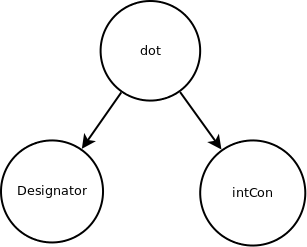
\includegraphics[width=0.4\textwidth]{./media/images/interpreter/syntaxbaum/designators/dot.png}

Dieser Knoten wird für Strukturen angewandt. Um die richtige Adresse für eine Variable in der Struktur zu bekommen, muss die Adresse des linken
Knotens mit der rechten Seite des Knotens addiert werden.

\begin{lstlisting}[language=JAVA]
return Adr(p.left) + p.right.val
\end{lstlisting}

\subsubsection{Index}
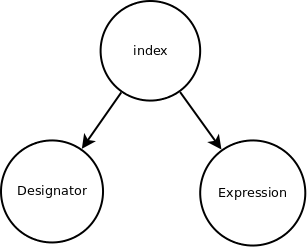
\includegraphics[width=0.4\textwidth]{./media/images/interpreter/syntaxbaum/designators/index.png}
Arrays werden vom Arrays verwendet. Um den Index des gewünschten Arrays auszurechnen, ist es notwendig, die Expression des rechten Knotens aufzulösen.
Nun kann die Adresse berechnet werden. Diese setzt sich aus dem Produkt der Adresse des rechten Knotens und der  Speicherbedarf eines einzelnen Indexelementes zusammen.

\begin{lstlisting}[language=JAVA]
return Adr(p.left) + p.left.type.elemType.size * index;
\end{lstlisting}

\subsection{Expressions}
Expressions werden grundsätzlich für Berechnungen und Typconvertierungen verwendet, aus diesem Grund ist es wichtig, dass jeder Datentyp seine eigene Expressions-Methode besitzt. Weiters können hier Konstanten abgefragt werden.

\subsection{Conditions}
Conditions werden für Vergleiche und für die Verwendung von if-Bedingungen sowie Schleifen benötigt. Weiters dienen sie auch zum verknüpfen mehrerer Conditions.

Hier wird unterschieden zwischen:
\begin{itemize}
\item EQL: Überprüft ob das Element auf der rechten Seite gleich dem der Linken Seite ist.
\item NEQ: Die Variable des Linken Knotens darf die des rechten Knotens nicht gleichen.
\item LSS: Das Element der Linken Seite muss kleiner sein als das der Rechten.
\item LEQ: Die Variable des Linken Knotens darf gleich, und kleiner sein als die Variable des Rechten.
\item GTR: Gibt true zurück, wenn die Variable des Linken Knotens größer ist als die des Rechten Knotens.
\item GEQ: Überprüft ob das Element auf der rechten Seite gleich oder größer dem der Linken Seite ist.
\item OR: Überprüft zwei Conditions mithilfe eines oder Operators.
\item AND: Zwei Conditions werden hiermit mit einem und verknüpft.
\item NOT: Der gegebene Linke Knoten ist eine Condition. Diese wird negiert zurückgegeben.
\item CALL: Ruft ein Unterprogramm auf, welches den Rückgabewert, den Datentyp Boolean hat. Dies kann somit für eine Abfrage weiterverwendet werden.
\end{itemize}
%	--------------------------------------------------------
% 	Kalkulation
%	--------------------------------------------------------
\section{Kalkulation}


%	--------------------------------------------------------
% 	Arbeitseinteilung
%	--------------------------------------------------------
\section{Arbeitseinteilung}

%	--------------------------------------------------------
% 	Compiler
%	--------------------------------------------------------	
%!TEX root = "../../DA_GUI.tex"

%	--------------------------------------------------------
% 	Aufbau der Benutzeroberfläche
%	--------------------------------------------------------

\chapter{Elemente der Benutzeroberfläche}
In diesem Kapitel wird der grundlegende Aufbau aller Fenster und Benutzeroberflächen von C Compact beschrieben - sowohl die konzeptuelle Konstruktion als auch die Implementierung.
\section{Das Konzept}
Die Erscheinung und Bedienung von C Compact folgt durchgehend der grundlegenden Idee, eine einfach und intuitiv zu bedienende Entwichlungsumgebung zu schaffen. Das bedeutet, Features möglichst Zielgruppenorientiert zu integrieren und überflüssige Funktionen zu vermeiden. Durch besondere Rücksicht auf Vollständigkeit und logische Bedienvorgänge haben wir ein durchgängig logisches Bedienerlebnis angestrebt.
Konkret haben wir uns dabei an folgende Ŕegeln gehalten:
\begin{itemize}
\item Das Erscheinen von Elementen in der Benutzeroberfläche soll logisch begründbar und verständlich vermittelbar sein
\item Funktionen, die im FSST-Unterricht der ersten und zweiten Klassen wahrscheinlich nicht benötigt werden, werden vermieden oder sind standardmäßig deaktiviert; Bedienelemente werden also auf das wesentlichste reduziert
\item Wir sind der Meinung, dass eine intuitiv zu bedinenede Oberfläche nicht durch Animationen und große Symbole erzeilt werden kann, sondern durch einfache, bereits bekannte Konzepte. So sind in C Compact bekannte Elemente wie beispielsweise eine Menüleiste mit gewohnten Datei- und Dokumentoperationen zu finden (Siehe Kapitel \ref{sec:gui-main-menu}).
%TODO reference GUImain
\end{itemize}

\subsection{Daraus resultierende Einschränkungen}
Durch diese Reduktion der gesamten Oberfläche ist C Compact auf einen bestimmten Zweck, also die Ausbildung, beschränkt. Das sehen wir allerdings nicht als Nachteil, sondern als besondere Stärke. Mit C Compact wollen wir eine Entwicklungsumgebung schaffen, die Anfänger nicht überfordert und ihnen hilft, sich auf das wesentliche zu konzentrieren.
Das Konzept einer anfängerfreundlichen Entwichlungsumgebung ist mit dem Aufbau einer Umgebung für die professionelle Entwicklung nicht vereinbar. C Compact soll aber auf späteres Arbeiten mit komplexeren Programmen vorbereiten. Schüler, die ihre erste Programmiersprache mit C Compact erlernen, kennen bereits den Umgang mit einem Debugger und haben ein tieferes verständnis für den Ablauf von Programmen.

%TODO add window desc. for launcher, quest seleter, package selecter
\section{Elemente und Fenster Der Benutzeroberfläche}
Neben dem Hauptfenster, das den Kern der Benutzeroberfläche darstellt, gibt es eine Reihe von kleineren Aktionsfenster, Dialogen und Einstellungsfenstern, die zum reibungslosen Ablauf bei der Bedienung von C Comapct beitragen. Das Hauptfenster selbst wird in Kapitel \ref{sec:gui-main} beschrieben.

\subsection{Launcher}
\label{sec:win-launcher}
...

\subsection{Einstellung der Sprache}
\label{sec:win-lang}
Wenn C Compact zum ersten Mal gestartet wird, wird zu allererst dieses fenster angezeigt. Der Benutzer wird gebeten, eine Sprache zu wählen. Später kann die Sprache über das Menü ,,Datei'' im Hauptfenster (Siehe Kapitel \ref{sec:gui-main-menu-file}) geändert werden. Die Änderungen werden erst wirksam, wenn der Benutzer die neue Sprache mit ,,OK'' bestätigt. Dann wird C Compact neu gestartet.
%TODO ref translations, Sprache

\begin{figure}[htp]
\centering

\includegraphics[width=0.3\textwidth]{./media/images/gui/elements/Bildschirmfoto-Sprache.png}
\caption{Auswahl der Sprache}
\label{fig:win-lang}
\end{figure}

Dieses Fenster ist in der Klasse \textbf{GUILanguage} im Package \textbf{at.jku.ssw.cmm.gui.properties} implementiert. 

\subsection{Allgemeine Einstellungen}
\label{sec:win-set}
Dieses Fenster enthält allgemeine Optionen zum Haupfenster der Benutzeroberfläche. Es kann im Menü des Hauptfensters unter ,,Datei'' -> ,,Einstelungen'' aufgerufen werden (Siehe Kapitel \ref{sec:gui-main-menu-file}). Änderungen an den Einstellungen werden sofort wirksam (ausgenommen sind Änderungen an der Schriftgröße von Dokumenten). Da C Compact beim Ändern dieser Einstellungen nicht neu gestartet werden muss, sind diese Optionen und die Spracheinstellungen in zwei unterschiedliche Fenster aufgeteilt.
%TODO ref GUImainSettings

\begin{figure}[htp]
\centering
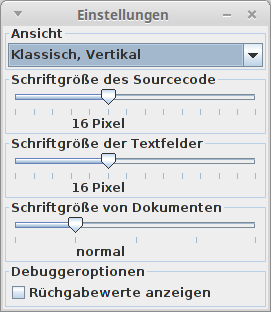
\includegraphics[width=0.4\textwidth]{./media/images/gui/elements/Bildschirmfoto-Einstellungen.png}
\caption{Einstellungsfenster}
\label{fig:win-set}
\end{figure}

Im Einstellungsfenster können folgende Optionen verändert werden:
\begin{enumerate}
\item \textbf{Ansicht:} Ändert den Aufbau des Hauptfensters. Elemente werden je nach gewähltem Layout unterschiedlich angeordnet. Siehe Kapitel \ref{sec:gui-main-left-ord}.
\item \textbf{Schriftgröße des Sourcecode:} Ändert die Schriftgröße des Textfeldes für den Sourcecode im Hauptfenster. Siehe Kapitel \ref{sec:gui-main-left-code}.
\item \textbf{Schriftgröße der Textfelder:} Ändert die Schriftgröße der Textfelder für Ein- und Ausgabedaten im Hauptfenster. Siehe Kapitel \ref{sec:gui-main-left-io}.
\item \textbf{Schriftgröße von Dokumenten:} Dokumente, wie etwa Beschreibungstexte von Fehlern, können mit unterschiedlichen Textgrößen angezeigt werden. Da die Schriftgröße beim Initialisieren der Textfelder festgelegt wird, betrifft die Einstellung immer nur die Dokumente, die in Zukunft geöffnet werden.
%TODO ref Fehlerdokumente
\item \textbf{Rückgabewerte anzeigen:} Hier kann eine Funktion des Debuggers aktiviert werden, die noch nicht ausgereift und auch nicht immer hilfreich ist: Wenn das Programm aus einer Funktion zurückspringt und in die Aufrufzeile einen Rückgabewert übergibt, wird dieser in einem Popup dargestellt.
%TODO Absatz nochmal lesen
%TODO ref popup
%TODO ref return popup
\end{enumerate}

Alle Klassen des Einstellungsfensters befinden sich im Package \textbf{at.jku.ssw.cmm.gui.properties}. Das Fenster selbst wird in der Klasse \textbf{GUIProperties} initialisiert, Listener für alle Schieberregler befinden sich in der Klasse \textbf{PropertiesSliderListener}. Die Combobox für das Layout der Benutzeroberfläche (Option 1) wird mit der Klasse \textbf{PropertiesComboListener} überwacht, die Checkbox für das Anzeigen von Rückgabewerten im Debugger ist mit dem ActionListener \textbf{PropertiesActionListener} verknüpft.

Beim Ändern der Schriftgröße werden zuerst die Einstellungen von C Compact verändert, dann werden die Schriftgrößen in den entsprechenden Elementen aktualisiert.
\begin{lstlisting}[language=JAVA]
@Override
public void stateChanged(ChangeEvent e) {
	JSlider slider = (JSlider)e.getSource();
	
	// Einstellungen aktualisieren
	main.getSettings().setCodeSize(GUIProperties.sliderPosToFont(slider.getValue()));
	
	// Schriftgrößen aktualisieren
	master.updateTextSize();
}
\end{lstlisting}

Tatsächlich wird beim aktuakisieren der Schriftgrößen einfach ein neuer Font mit der entsprechenden Größe aus dem bereits verwendeten Font abgeleitet und angewandt.
%TODO ref GUIleftPanel
\begin{lstlisting}[language=JAVA]
// Schriftart (font) ändern
this.jSourcePane.setFont(
	// Aktuellen Font ableiten
	this.jSourcePane.getFont().deriveFont(
		//Schriftgröße laut Einstellungen
		(float)this.main.getSettings().getCodeSize()
	)
);
\end{lstlisting}

Die Schriftgröße von Dokumenten wird, wie in Punkt 4 bereits erwähnt, beim laden des Dokumentes festgelegt.
%TODO ref Dokumente laden

\subsection{Über C Compact}
% !!! TODO mention SSW in credits !!!
Dieses Fenster enthält den Lizenztext von C Compact sowie die Namen der beteiligten Personen. Auch dieses Fenster kann im Menü der Entwicklungsumgebung aufgerufen werden (Menü siehe Kapitel \ref{sec:gui-main-menu-file}). Alle Bestandteile dieses Elementes befinden sich im Package \textbf{at.jku.ssw.cmm.gui.credits}:
\begin{itemize}
\item \textbf{Credits.java:} Initialisiert das Fenster und regelt sein Verhalten.
\item \textbf{credits.html:} Enthält den Lizenztext.
\item \textbf{credits.css:} Enthält formatierungsinformationen zum Lizenztext.
\end{itemize}
%TODO ref Dokumente laden

Die Resourcen sind im Package eingebunden und deshalb auch Teil der generierten JAR-Datei. Dadurch kann der Lizenztext nicht einfach verändert werden.

\begin{figure}[htp]
\centering
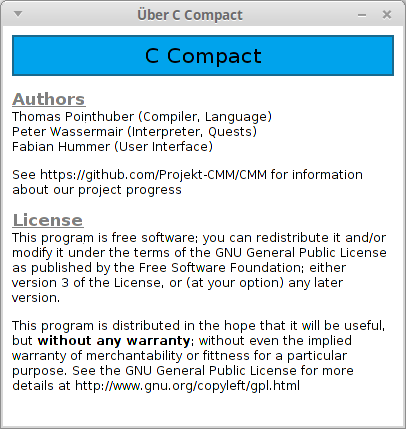
\includegraphics[width=0.4\textwidth]{./media/images/gui/elements/Bildschirmfoto-About.png}
\caption{Fenster mit Lizenztext}
\label{fig:win-about}
\end{figure}

\subsection{Questpacket auswählen}
...

\subsection{Quest auswählen}
...

\subsection{Profil erstellen}
... name eingeben ...

\subsection{Dialoge}
In C Compact werden viele verschiedene Dialogfenster verwendet. Der Begriff Dialogfenster\footnote{http://de.wikipedia.org/wiki/Dialog\_(Benutzeroberfläche)} umfasst eine Reihe von unterschiedlichen Anwendungen, bei denen ein Fenster werwendet wird, um Informationen oder Befehle vom Benutzer einzuholen. Dialoge werden in C Compact beispielsweise verwendet, um zu fragen, ob eine Datei gespeichert werden soll (Abbildung \ref{fig:win-dialog}), oder um den Benutzer auf ein Problem aufmerksam zu machen. Swing enthält bereits einige Funktionen zum Erstellen von Dialogen\footnote{http://docs.oracle.com/javase/tutorial/uiswing/components/dialog.html}, anhand dieses Tutorials können einfache Dialoge sehr schnell erstellt werden.

\begin{figure}[htp]
\centering
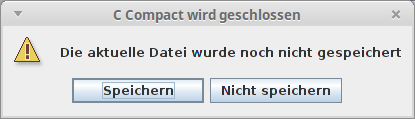
\includegraphics[width=0.4\textwidth]{./media/images/gui/elements/Bildschirmfoto-Dialog.png}
\caption{Ein einfacher Dialog}
\label{fig:win-dialog}
\end{figure}

\subsection{Dateimanager}
...

%TODO add information about info saved in profiles
\section{Einstellungen}
Für den Betrieb einer fortgeschrittenen Benutzeroberfläche ist es unerlässlich, diese anpassbar zu machen und Anpassungen des Benutzers zu speichern. Im Package \textbf{at.jku.ssw.cmm.gui.properites} befindet sich die Klasse \textbf{GUImainSettings}, die alle globalen Einstellungen überwacht. Diese Einstellungen umfassen:
\begin{itemize}
\item Die zuletzt geöffneten Dateien
\item Die gerade geöffnete Datei
\item Die zuletzt geöffneten Benutzerprofile
\item Das aktuell aktive Benutzerprofil
\item Die vom Benutzer gewählte Sprache
%TODO ref language
\item Einstellungen, die der Benutzer direkt verändern kann (Siehe Kapitel \ref{sec:win-set})
\begin{itemize}
\item Schriftgrößen
\item Layout der Benutzeroberfläche
\end{itemize}
\end{itemize}

Bevor das Hauptfenster der Entwicklungsumgebung gestartet werden kann, muss ein Objekt der Klasse \textbf{GUImainSettings} erstellt werden (Siehe dazu Kapitel \ref{sec:gui-main-impl}). Dabei werden die zuletzt gespeicherten Einstellungen geladen.

Die Einstellungen werden in der Datei \textbf{settings.xml} im Hauptverzeichnis von C Compact gespeichert. Bevor diese Datei ausgelesen wird, werden alle Einstellungsvariablen auf einen definierten Standardwert gesetzt. Sollten also bestimmte Informationen oder alle Einstellungen fehlen, werden die Standardwerte wieder hergestellt. Die Einstellungen werden beim Beenden von C Comapct gespeichert.

Die Einstellungsdatei \textbf{settings.xml} ist wie folgt aufgebaut:
\begin{lstlisting}[language=XML]
<?xml version="1.0" encoding="UTF-8" standalone="no"?>
<settings xmlns="settings.xml">
	<properties>
		<language>de</language>
		<codesize>16</codesize>
		<textsize>16</textsize>
		<varsize>16</varsize>
		<varoffset>0</varoffset>
		<descsize>0</descsize>
		<returnpopup>false</returnpopup>
	</properties>
	<lastfile>/home/fabian/Dokumente/C--/C_Compact_Alpha_1.4.5/examples/helloworld/helloworld.cmm</lastfile>
	<lastfile>/home/fabian/Dokumente/C--/C_Compact_Alpha_1.4.5/examples/random/random.cmm</lastfile>
	<lastfile>/home/fabian/Dokumente/C--/C_Compact_Alpha_1.4.5/examples/bubblesort/bubblesort.cmm</lastfile>
	<profile>/home/fabian/Dokumente/profile_Fabian</profile>
</settings>
\end{lstlisting}

Unter ,,properties'' befinden sich alle Parameter, die der Benutzer direkt einstellen kann (die Sprache bei den Spracheinstellungen, siehe Kapitel \ref{sec:win-lang} und alle anderen Einstellungen bei den allgemeinen Einstellungen, siehe Kapitel \ref{sec:win-set}). Darunter werden die zuletzt gewählten Profile aufgelistet (diese werden im Launcher angezeigt, siehe Kapitel \ref{sec:win-launcher}) und dann die zuletzt geöffneten Dateien (für die Auflistung im Menü der Entwicklungsumgebung, siehe Kapitel \ref{sec:gui-main-menu-ctrl}). Damit die Listen nicht zu lang werden, werden nur die letzten 10 geöffneten Dateien und die letzten 10 aktiven Profile gespeichert und angezeigt.
%TODO appendix: how to read XML file



%	--------------------------------------------------------
% 	Projektbeschreibung
%	--------------------------------------------------------	
%%!TEX root=../Vorlage_DA.tex
%	########################################################
% 				Projektbeschreibung
%	########################################################


%	--------------------------------------------------------
% 	Überschrift, Inhaltsverzeichnis
%	--------------------------------------------------------
\chapter{Projektbeschreibung}

%	--------------------------------------------------------
% 	Interpreter
%	--------------------------------------------------------
\section{Compiler}

%!TEX root=../Vorlage_DA.tex
%	########################################################
% 				Projektbeschreibung
%	########################################################


%	--------------------------------------------------------
% 	Überschrift, Inhaltsverzeichnis
%	--------------------------------------------------------
\chapter{Compiler}

%	--------------------------------------------------------
% 	Allgmeine Hinweise
%	--------------------------------------------------------
%!TEX root=../Vorlage_DA.tex
%	########################################################
% 				Allgemeiner Teil (Theorie)
%	########################################################


%	--------------------------------------------------------
% 	Allgmeine Hinweise
%	--------------------------------------------------------
\section{Allgemeiner Teil (Theorie)}

\subsection{Erweiterte Backus-Naur-Form (EBNF)}

Die sogenannte Erweiterte Backus-Naur-Form (EBNF)\footnote{\url{https://de.wikipedia.org/wiki/Erweiterte_Backus-Naur-Form}} ist eine weiterentwicklung der Backus-Naur-Form (BNF)\footnote{\url{https://de.wikipedia.org/wiki/Backus-Naur-Form}}. Das Anwendungsgebiet der BNF und EBNF ist das definieren von  kontextfreie Grammatiken\footnote{\url{https://de.wikipedia.org/wiki/Kontextfreie_Grammatik}}, welche untere anderem f\"ur Programmiersprachen benutzt werden.

Bei kontextfreier Gramatik wird jeweils Ein Nichtterminalsymbol auf eine beliebige Folge von Terminal- bzw. Nichtterminalsymbolen abgeleitet ($V \rightarrow w$). Wenn das Nichtterminalsymbol $V$ in einem anderem Nichtterminalsymbol verwendet wird, wird nicht auf den Kontext geachtet, in welcher das Nichtterminalsymbol $V$ eingebettet ist. Die Regel ist daher kontextfrei.

Vorteile der EBNF gegen\"uber der BNF sind unter anderem:

\begin{itemize}
  \item einfacheres erstellen von Rekursionen und optionalen Ausdr\"ucken
  \item bessere Lesbarkeit
  \item einfaches und eindeutiges Definieren von Terminalsymbolen
\end{itemize}

\newpage

\subsubsection{Terminalsymbol}

Ein sogenanntes Terminalsymbol\footnote{\url{https://de.wikipedia.org/wiki/Terminalsymbol}} wird nicht weiter zerlegt. Es stellt z.B. eine Zahl, eine Variable oder ein Schlüsselwort (''if'', ''while'', ...) dar.

\begin{lstlisting}[language=EBNF]
Expr = Term { ( "+" | "-" ) Term }.
Term = intCon { ( "*" | "/" ) intCon }.
\end{lstlisting}

Terminalsymbole werden normalerweise entweder klein geschrieben (z.B. intCon), oder direkt in der Gramatik definiert (z.B. ''+'').

\subsubsection{Nichtterminalsymbol}

Ein Nichtterminalsymbol\footnote{\url{https://de.wikipedia.org/wiki/Nichtterminalsymbol}} besteht aus einen oder mehreren Terminalsymbolen bzw. Nichtterminalsymbolen.

\begin{lstlisting}[language=EBNF]
Expr = Term { ( "+" | "-" ) Term }.
Term = intCon { ( "*" | "/" ) intCon }.
\end{lstlisting}

Nichtterminalsymbole werden normalerweise gro\ss{} geschrieben. In diesem Beispiel stellen ''Expr'' und ''Term'' Nichtterminalsymbole dar, welche wiederum von anderen Nichtterminalsymbolen verwendet werden k\"onnen.

\subsubsection{Produktionsregel}

Die Produktionsregel\footnote{\url{https://de.wikipedia.org/wiki/Produktionsregel}} ist eine Regel, welche angibt wie aus W\"ortern neue W\"orter produziert werden.

\begin{lstlisting}[language=EBNF]
Expr = Term { ( "+" | "-" ) Term }.
Term = intCon { ( "*" | "/" ) intCon }.
\end{lstlisting}

Die Produktionsregel gibt an wie z.B. das Nichtterminalsymbol ''Expr'' aufgebaut ist. Eine Produktionsregel besteht jeweils aus einem Nichtterminalsymbol auf der linken Seite, und der jeweiligen Regel auf der rechten Seite welches aus Terminal- und Nichtterminalsymbolen aufgebaut ist.

\newpage

\subsubsection{Eindeutigkeit}

Die Gramatik muss so aufgebaut sein, dass es für einen Tokenstrom nur eine eindeutige Möglichkeit gibt diesen zu parsen.\footnote{\url{http://www.iai.uni-bonn.de/III//lehre/vorlesungen/Informatik_I/WS05/Folien/VLWS0506-10.pdf}}

\htlParagraph{Beispiel}

Es soll eine EBNF-Regel erstellt werden welche einen Mathematischen Ausdruck, aufgebaut aus Additionen und Subtraktionen korrekt parsen.
\subhtlParagraph{Mehrdeutige EBNF Regel}

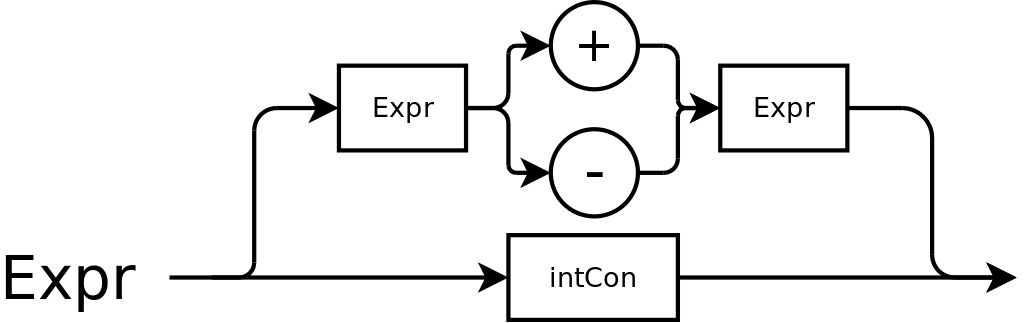
\includegraphics[width=0.6\textwidth]{./media/images/compiler/ambiguity_wrong.png}

\begin{lstlisting}[language=EBNF]
Expr = intCon | Expr ( "+" | "-" ) Expr.
\end{lstlisting}

Der Ausdruck $1-2+5$ kann mit dieser EBNF Regel auf mehreren Arten gelöst werden. Es liegt also eine Mehrdeutigkeit vor. Der Ausdruck $1-2+5$ kann dabei sowohl als $(1-2)+5$, aber auch als $1-(2+5)$ geparst werden.

\begin{tabular}{ c | c }
  $(1-2)+5=4$ & 
  $1-(2+5)=-6$ \\
  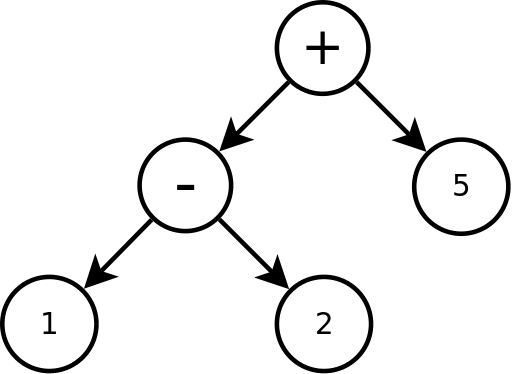
\includegraphics[width=0.2\textwidth]{./media/images/compiler/ambiguity_tree_correct.png} & 
  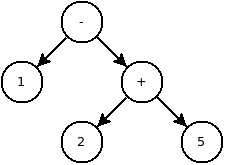
\includegraphics[width=0.2\textwidth]{./media/images/compiler/ambiguity_tree_wrong.png} \\
\end{tabular}
\subhtlParagraph{Eindeutige EBNF Regel}

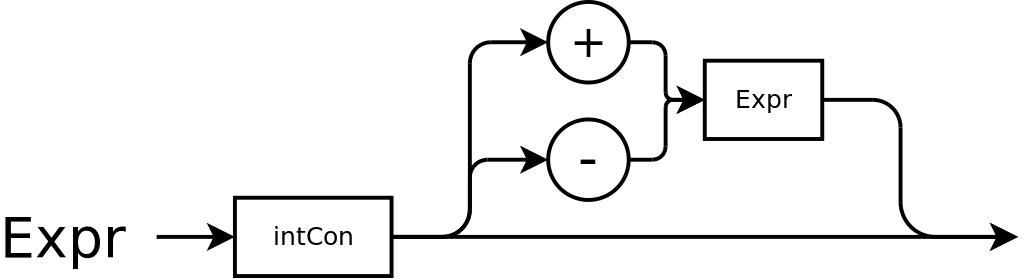
\includegraphics[width=0.6\textwidth]{./media/images/compiler/ambiguity_correct.png}

\begin{lstlisting}[language=EBNF]
Expr = intCon [ ( "+" | "-" ) Expr ].
\end{lstlisting}

Der Ausdruck $1-2+5$ kann mit dieser EBNF Regel nur mehr auf eine Art gelöst werden. Dabei werden die Operatoren links-assoziativ behandelt. Der Ausdruck $1-2+5$ wird als $(1-2)+5$ ausgewertet, was Mathematisch den korrekte Weg darstellt.

\subsubsection{EBNF-Beispiele}

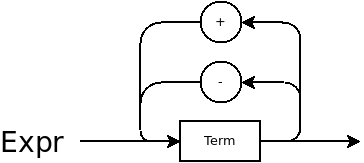
\includegraphics[width=0.5\textwidth]{./media/images/compiler/ebnf_expr.png}

\begin{lstlisting}[language=EBNF]
Expr = Term { ( "+" | "-" ) Term }.
\end{lstlisting}

Eine Expression\footnote{\url{https://de.wikipedia.org/wiki/Ausdruck_(Programmierung)}} besteht dabei aus einem Term, und dann optional wiederum aus einem ''+'' oder ''-'' gefolgt von einem weiterem Term.

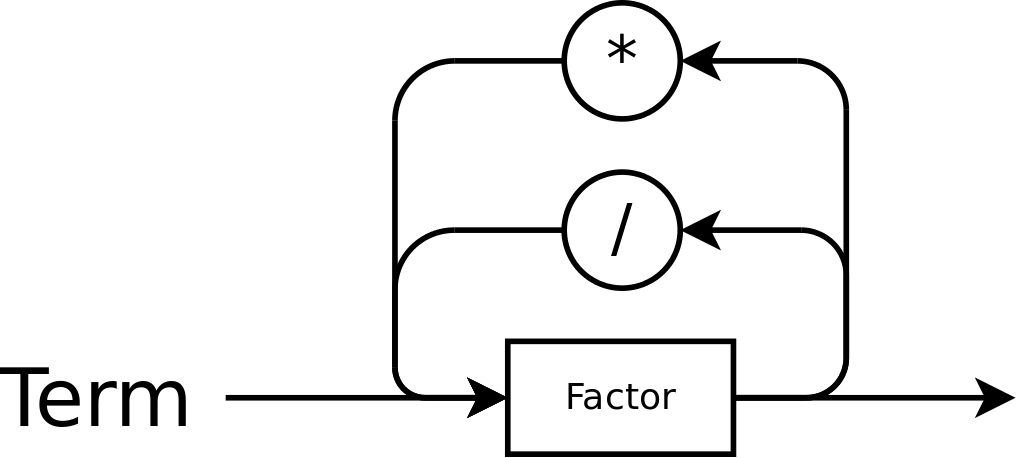
\includegraphics[width=0.5\textwidth]{./media/images/compiler/ebnf_term.png}
\begin{lstlisting}[language=EBNF]
Term = Factor { ( "*" | "/" ) Factor }.
\end{lstlisting}

Das Nichtterminalsymbol Term stellt wiederum eine Produktionsregel dar, welche aus einem Faktor, und dann optional wiederum aus einem ''*'' oder ''/'' gefolgt von einem weiterem Faktor besteht.

Durch solche einfachen Regeln können z.B.: Mathematische Regeln wie Punkt vor Strich eindeutig und korrekt in einen Syntaxbaum übersetzt werden.

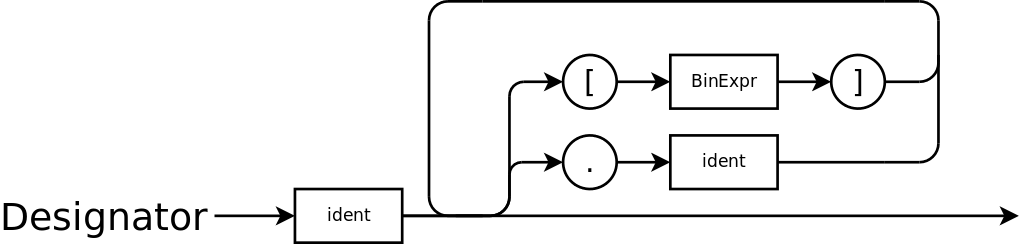
\includegraphics[width=\textwidth]{./media/images/compiler/ebnf_designator.png}
\begin{lstlisting}[language=EBNF]
Designator = ident { "." ident | "[" BinExpr "]" }.
\end{lstlisting}

%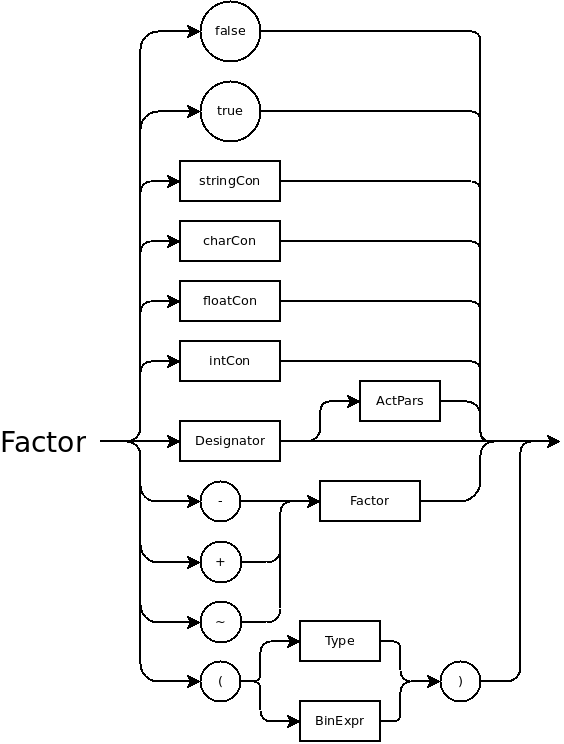
\includegraphics[width=0.6\textwidth]{./media/images/compiler/ebnf_factor.png}

\newpage

\subsection{Lexikalische Analyse - Scanner}

Bei der Lexikalischen Analyse zerlegt der sogenannt Scanner\footnote{\url{https://de.wikipedia.org/wiki/Tokenizer}} den Zeichenstrom in einen sogenannten Tokenstrom. Ein sogenannter Token\footnote{\url{https://de.wikipedia.org/wiki/Token_(\%C3\%9Cbersetzerbau)}} stellt dabei eine logische Einheit dar (z.B.: eine variable, oder ein Operatorzeichen), und wird nicht mehr weiter zerlegt (Terminalsymbol).

\htlParagraph{Zeichenstrom}

Der Scanner bekommt einen Zeichenstrom, welcher aus einzelnen Zeichen besteht. Ein Zeichen ist z.B. ein Buchstabe, eine Zahl oder Sonderzeichen wie ''='', oder ''+''.


\includegraphics[width=0.6\textwidth]{./media/images/compiler/input_characterstream.png}

\htlParagraph{Resultierender Tokenstrom}

Aus diesem Zeichenstrom werden dann die Tokens extrahiert, welche dann die sogenannten Terminalsymbole in der EBNF bzw. BNF darstellen. Tokens k\"onnen dabei aus 1. oder mehreren Zeichen bestehen.

Manche Tokens wie z.B. Variablen oder Konstanten besitzen au\ss{}er der Tokennummer desweiteren noch einen Tokenwert, mit dem sp\"ater z.B. der Variablenname, oder der Wert einer Variable ausgelesen werden kann.

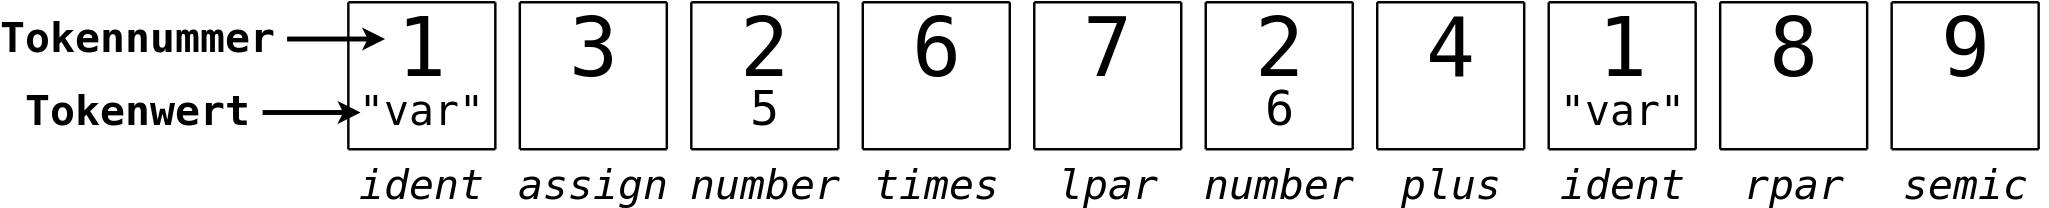
\includegraphics[width=\textwidth]{./media/images/compiler/scanner_tokenstream.png}

\subsection{Syntaxanalyse - Parser}

Der Parser\footnote{\url{https://de.wikipedia.org/wiki/Parser}} wandelt danach den Tokenstrom in einen Syntaxbaum um, welcher das Programm repräsentiert.

Es gibt verschiedene Verfahren um dies zu bewerkstelligen. Wir verwenden f\"ur unser Projekt Coco/R\footnote{\url{https://de.wikipedia.org/wiki/Coco/R}}, welcher einen LL(k)\footnote{\url{https://de.wikipedia.org/wiki/LL(k)-Grammatik}} Parser implementiert, wobei im Normalfall $k = 1$ ist. Falls $k > 1$ ist, muss f\"ur diesen Fall eine eigene Funktion implementiert werden, welche entscheidet wie der Parser weiterarbeiten soll.

Ein LL(1) Parser arbeitet dabei so, dass er jeweils um 1. Token nach vorne schaut, und mithilfe dieser Information den weiteren Parservorgang steuert.

% http://amor.cms.hu-berlin.de/~kunert/papers/lr-analyse/

\newpage

\htlParagraph{Syntaxbaum}

Der Parser \"ubersetzt den Tokenstrom in einen sogenannten Syntaxbaum\footnote{\url{https://de.wikipedia.org/wiki/Syntaxbaum}}, welcher die Struktur des Programmes repr\"asentiert.

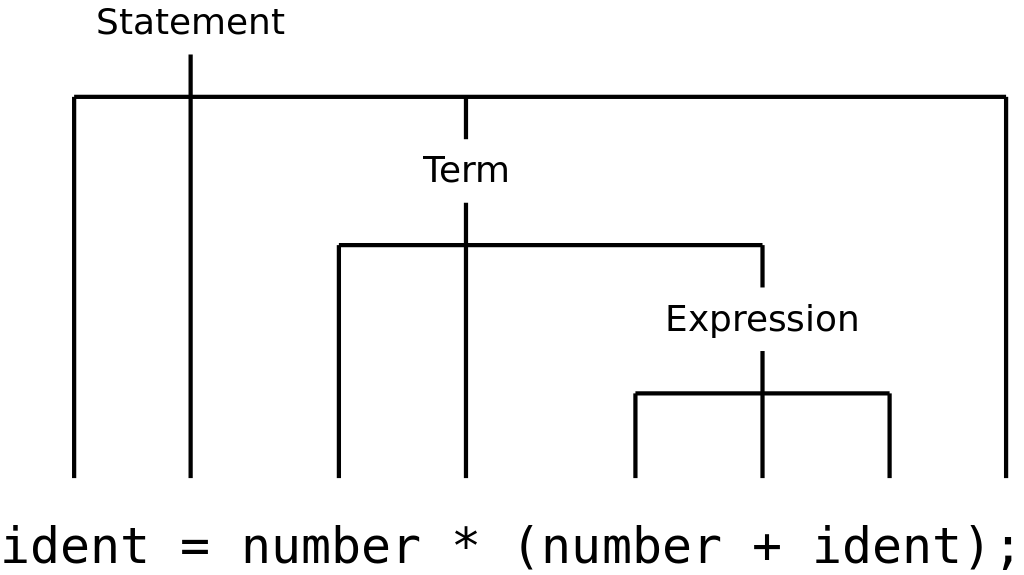
\includegraphics[width=0.6\textwidth]{./media/images/compiler/parser_syntaxtree.png}

\subsection{Abstrakter Syntaxbaum}

Der ''allgemeine'' Syntaxbaum enth\"alt viele unn\"otigen Daten, welche beim Abstraken Syntaxbaum\footnote{\url{https://de.wikipedia.org/wiki/Abstrakter_Syntaxbaum}} nicht mehr vorhanden sind. Der Abstrakte Syntaxbaum stellt somit eine Baumrepr\"asentation der wesentlichen Syntax eines Programmes dar.

\includegraphics[width=0.6\textwidth]{./media/images/compiler/abstract_syntaxtree.png}

\subsubsection{homogene und heterogene Syntaxbäume}

Der Abstrakte Syntaxbaum kann entweder aus einheitlichen Knoten (homogen) oder aus verschiedenen Knoten (heterogen) aufgebaut sein.\footnote{\url{https://wiki.fernuni-hagen.de/eclipse/index.php/Abstract_Syntax_Tree_(AST)\#Konzept_des_Syntaxbaums}}

\subsection{Attributierte Gramatik}

%\footnote{\url{https://de.wikipedia.org/wiki/Attributgrammatik}}
Bei der Attributierten Gramatik\footnote{\url{http://steffenpingel.de/files/papers/ast.pdf}} werden Berechnungsvorschriften direkt in die Gramatik eingef\"ugt. Dadurch k\"onnen w\"arend des Parsens unter anderem Syntaxbedingungen wie z.B. Typpr\"ufungen durchgef\"uhrt werden.

In Coco/R werden diese Berechnungsvorschriften mit ''(.'' eingeleitet und mit ''.)'' beendet. Zwischen diesen Klammern befindet sich dann der Quellcode, welcher ausgef\"uhrt wird, falls der Parser den Ausdruck durchl\"auft.

\htlParagraph{Beispiel}

\begin{lstlisting}[language=EBNF]
Type<out Struct type>
= 
ident     (.  // check if a type with the given name exist
              Obj obj = tab.find(t.val);
              if(obj.kind != Obj.TYPE)
                  SemErr(obj.name + " is not a type");

              type = obj.type; .)
. 
\end{lstlisting}

In diesem Beispiel pr\"uft die Berechnungsvorschrift ob bereits ein Identifier mit dem gew\"ahlten Namen definiert wurde (passiert in der Funktion tab.find(t.val);), und ob der gefundene Identifier ein Typ ist. 

Falls eine dieser Syntaxbedingungen fehlschl\"agt, wird ein Semantischer Fehler geworfen. So werden w\"ahrend des Parsens nicht nur Syntaxfehler, sondern auch logische Fehler detektiert (z.B. fehlende Variablendeklaration).

Desweiteren kann durch diese Berechnungsvorschriften ein Abstrakter Syntaxbaum aufgebaut werden. Eine EBNF-Regel stellt nicht unbedingt einen Knoten im Abstrakten Syntaxbaum dar, da z.b. Variablendeklarationen oft in sogenannte Symboltabellen gespeichert werden.

\subsection{Symboltabelle}

Die Symboltabelle\footnote{\url{https://de.wikipedia.org/wiki/Symboltabelle}} ist eine Datenstruktur in der Variablen und Funktionsdeklarationen gespeichert werden. Sie umfasst dabei Informationen wie z.b. Zeile, in der die Variable/Funktion deklariert wurde, die gr\"o\ss{}e des Datentypes, oder auch den Wert welchen mit welchem die Variable deklariert wurde (Konstanten).

Mithilfe der Symboltabelle wird unter anderem festgestellt, ob eine Variablen deklariert wurde, oder wie viel Speicher f\"ur eine Funktion reserviert werden muss.

%, und l\"ost m\"ogliche Namensprobleme auf.\footnote{\url{https://de.wikipedia.org/wiki/Namensraum}}

\subsection{Scope}

%	--------------------------------------------------------
% 	Lösungsansätze
%	--------------------------------------------------------
%%!TEX root=../Vorlage_DA.tex
%	########################################################
% 				Lösungsansätze
%	########################################################


%	--------------------------------------------------------
% 	Lösungsansätze
%	--------------------------------------------------------
\section{Lösungsansätze}


%	--------------------------------------------------------
% 	Realisierte Lösungen
%	--------------------------------------------------------
%!TEX root=../Vorlage_DA.tex
%	########################################################
% 				Realisierte Lösungen
%	########################################################


%	--------------------------------------------------------
% 	Realisierte Lösungen
%	--------------------------------------------------------
\section{Realisierte Lösungen}

%	--------------------------------------------------------
% 	EBNF
%	--------------------------------------------------------
\input{./chapters/compiler/03-01-ebnf.tex}

%	--------------------------------------------------------
% 	Lexikalische Struktur
%	--------------------------------------------------------
\input{./chapters/compiler/03-02-lexical_structure.tex}

%	--------------------------------------------------------
% 	Syntaxbäume
%	--------------------------------------------------------
\input{./chapters/compiler/03-03-syntaxtree.tex}

%	--------------------------------------------------------
% 	Standardbibliotek
%	--------------------------------------------------------
\input{./chapters/compiler/03-04-standard-library.tex}

\subsection{Kontextbedingungen}

\subsection{Typkonvertierung}

\subsection{Scope}

\subsection{Strings}

%	--------------------------------------------------------
% 	Sprachspezifikation
%	--------------------------------------------------------
%!TEX root=../Vorlage_DA.tex
%	########################################################
% 				Allgemeiner Teil (Theorie)
%	########################################################


%	--------------------------------------------------------
% 	Sprachspezifikation
%	--------------------------------------------------------
\newpage
\section{Sprachspezifikation}

\subsection{Pr\"aprozessor}

Unser Pr\"aprozessor erm\"oglicht die Nutzung mehrer Dateien und verf\"ugt \"uber die Funktion einzelne Codeteile zu deaktivieren, wie es auch in C der Fall ist. Pr\"aprozessorargumente beginnen dabei jeweils mit einem Hashtag, gefolgt von der jeweiligen Direktive und einem oder mehreren Argumenten.

\subsubsection{\#include Direktive}

Mithilfe eines \#include k\"onnen andere Dateien eingebunden werden. Es gibt dabei 2. Arten von \#include, welche sich durch den jeweiligen Suchpfad unterscheiden. Aus Technischer Sicht kopiert der Pr\"aprozessor die jeweilige Datei an die Stelle wo das \#include geschrieben ist.

\htlParagraph{Suche im Standard-Include-Pfad}

Der Standard-Include-Pfad stellt der Ordner clib dar, in welchem sich die Standardbibliothek befindet.

\begin{lstlisting}[language=C]
#include <stdio.h>
\end{lstlisting}

\htlParagraph{Suche im aktuellen Verzeichnis}

Wenn selbst geschriebene Programmdateien eingebunden werden sollen wird der Pfad relativ zum aktuellen Verzeichnis angegeben. So ist es m\"oglich gro\"o\ss{}ere Projekte auf Basis mehrere Dateien zu entwickeln.

\begin{lstlisting}[language=C]
#include "foo.cmm"
\end{lstlisting}

\subsubsection{\#define Direktive}

Es ist m\"oglich den w\"ahrend des Pr\"aprozessorvorganges Variablen zu definieren, welche aber nur im Pr\"aprozessor ausgewertet werden k\"onnen. Es ist nicht m\"oglich mithilfe eines \#define Quelltext zu ver\"andern, wie es in C m\"oglich ist!

Es ist m\"oglich einem Define einen Wert zuzuweisen, welcher eine Ganze Zahl sein muss. Falls kein Wert angegeben ist wird 1 angenommen.

\begin{lstlisting}[language=C]
#define __DEFINE_WITHOUT_VALUE__
#define __DEFINE_WITH_VALUE__ 0
\end{lstlisting}

Falls ein \#define mit dem gleichen Namen bereits existiert, wird dieses \"uberschrieben.

\subsubsection{\#undef Direktive}

Mithilfe eines \#undef kann eine definierte Variable gel\"oscht werden. Die Variable steht somit nicht mehr zur verf\"ugung, bis die Variable erneut definiert wird.

\begin{lstlisting}[language=C]
#undef __DEFINE_WHICH_IS_NOW_DELETED__
\end{lstlisting}

\subsubsection{\#ifdef, \#ifndef, \#else und \#endif Direktive}

Es ist m\"oglich abzufragen ob es eine bestimmte Variablendefinition gibt, oder nicht gibt. Diese Abfrage wird mit den Pr\"aprozessorargumenten \#ifdef bzw. \#ifndef eingeleitet, und muss mit einem \#endif enden. Falls es notwendig ist auch f\"ur das Gegenargument code auszuf\"uhren kann dies mithilfe eines \#else eingeleitet werden.

Eine Variable gilt als definiert wenn sie mithilfe eines \#define erzeugt wurde, und einen Wert ungleich 0 besitzt.

\begin{lstlisting}[language=C]
#ifdef __SOME_DEFINE__
	// ... Do something if __SOME_DEFINE__ is defined
#else
	// ... Do something if __SOME_DEFINE__ is not defined
#endif
\end{lstlisting}

\subsubsection{Beispiel}

Der Pr\"aprozessor wird besonders daf\"ur ben\"otigt, dass Bibliotheken bei mehrfachen \#include keine Fehler verursachen. Dazu ist es notwendig dass die Bibliothek bei mehrfachen \#include die nachfolgenden Ignoriert. Dies stellt ein Standardkonstrukt in der C Programmierung dar.

\begin{lstlisting}[language=C]
#ifndef __CLIB_EXAMPLE__

	#define __CLIB_EXAMPLE__
	
	// ... some includes if required
	#include <stdio.h>

	// ... here is the executed code of the file

#endif /* __CLIB_EXAMPLE__ */
\end{lstlisting}

Zuerst wird ermittelt, ob die Bibliothek bereits eingebunden wurde (falls dies der Fall ist, ist die jeweilige Variable definiert), und \#ifndef ignoriert infolge den folgenden Code bis zum \#endif.

Falls der Code aber das erste mal eingebunden wurde, ist die Variable (in diesem Beispiel $\_\_CLIB\_EXAMPLE\_\_$) noch nicht definiert worden. Folglich wird der Code welcher sich in \#ifndef befindet ausgef\"uhrt, wo unter anderem die jeweilige Variable definiert wird, welche einzigartig f\"ur die jeweilige Bibliothek sein muss.

\subsection{Kommentare}

Bereiche welche als Kommentar\footnote{\url{https://de.wikipedia.org/wiki/Kommentar_(Programmierung)}} deklariert sind, werden vom Pr\"aprozessor und vom Compiler ignoriert. Es gibt dabei 2. Arten von Kommentare.

\htlParagraph{Zeilenkommentar}

Ein Zeilenkommentar beginnt mit einem //, und endet mit dem Ende der Zeile.

\begin{lstlisting}[language=C]
// this is a simple line comment
\end{lstlisting}

\htlParagraph{Blockkommentar}

Ein Blockkommentar beginnt mit einem /* und enden bei dem ersten auftreten eines */.

\begin{lstlisting}[language=C]
/* this is a
   blockcomment */
\end{lstlisting}

\subsection{Datentypen}

Der gew\"ahlte Datentyp\footnote{\url{https://de.wikipedia.org/wiki/Datentyp}} gibt an welche Art von Daten gespeichert werden k\"onnen. Es gibt primitive Datentypen, welche gro\"ss{}teils auch Arithmetische Datenoperationen unterst\"utzen, und Zusammengesetzte Datentypen welche aus einem oder mehreren primitiven Datentypen aufgebaut sind.

\subsubsection{Primitive Datentypen}

\htlParagraph{void}

void bezeichnet keinen eigentlichen Typen, und ist nur f\"ur die Definition von Funktionen erlaubt, welche nichts zur\"uckgeben.

\begin{lstlisting}[language=C]
void foo() {
}
\end{lstlisting}

\htlParagraph{bool}

bool unterst\"utzt die beiden Wahrheitswerte true und false. Wenn ein int als bool ausgewertet wird, stellt 0 false dar, und ungleich 0 ist true.

\begin{lstlisting}[language=CMM]
bool b;

bool foo() {
	return true;
}
\end{lstlisting}

\htlParagraph{char}

Ein char stellt ein einzelnes alphanumerisches Zeichen, ein Leerzeichen oder das Sonderzeichen \textbackslash{}r, \textbackslash{}n, \textbackslash{}t, \textbackslash{}0, \textbackslash{}' oder \textbackslash{}\textbackslash{} dar.

\begin{lstlisting}[language=CMM]
char ch;

char foo() {
	return 'c';
}
\end{lstlisting}

\htlParagraph{int}

Ein int stellt eine ganzzahlige Zahl dar, welche einen Wert zwischen $-2147483648$ und $2147483647$ haben muss.

\begin{lstlisting}[language=CMM]
int i;

int foo() {
	return 1234;
}
\end{lstlisting}

\htlParagraph{float}

\begin{lstlisting}[language=CMM]
float f;

float foo() {
	return 1.2;
}
\end{lstlisting}

\htlParagraph{string}

\begin{lstlisting}[language=CMM]
string s;

string foo() {
	return "Hello World";
}
\end{lstlisting}

\subsubsection{Konstanten}

Konstanten sind Variablen, welche nicht ver\"andert werden k\"onnen. Der Wert muss dabei bei der Deklaration angegeben werden, und muss dem Datentyp der Konstante entsprechen (Typumwandlungen sind nicht zul\"assig!).

\begin{lstlisting}[language=CMM]
const int i = 1234;
\end{lstlisting}

\subsubsection{Strukturen}

Strukturen sind zusammengesetzte Datentypen welche aus 1. oder mehreren Datentypen bestehen. Eine definierte Struktur stellt einen neuer Datentyp dar, von welchem Variablen definiert werden k\"onnen, welche man auch an Funktionen \"ubergeben kann.

Strukturen k\"onnen nicht auf sich selbst verweisen, da es ansonsten eine endlosen Rekursion darstellen w\"urde. Des weiteren k\"onnen keine Werte bei der Definition einer Struktur angegeben werden.

\begin{lstlisting}[language=CMM]
struct Point {
    int x, y;
    string name;
}

Point p;
\end{lstlisting}

\subsubsection{Arrays}

Arrays sind Felder von Datentypen, wobei ein einzelnes Feld mithilfe eines sogenannten Index spezifiziert werden kann.

Falls ein Array in einer Funktion definiert wird, kann diesem ein Initialisierungswert zugewiesen werden, welcher das Array mit definierten Werten f\"ullt.

\begin{lstlisting}[language=CMM]
char cArr[10];
int arr[5][5];
\end{lstlisting}

\subsubsection{Typumwandlung}

Es ist m\"oglich Datentypen in einen anderen Umzuwandeln. Dies kann einerseits implizit geschehen, oder muss explizit angegeben werden. Es ist nicht m\"oglich jeden Datentyp in jeden anderen umzuwandeln. Strukturen und Arrays können bis auf besondere ausnahmef\"alle nicht umgewandelt werden.

\htlParagraph{Implizite Typumwandlung}

Bei der Impliziten Typumwandlung wird diese automatisch w\"ahrend des Compiliervorganges durchgef\"urt.

\begin{lstlisting}[language=CMM]
float f = 1 + 2.5; // 1 is implicit converted to float
\end{lstlisting}

\htlParagraph{Explizite Typumwandlung}

Die explizite Typumwandlung ist besonders dann notwendig, falls ein Datentyp in einen anderen umgewandelt werden muss, welcher weniger Daten speichern kann als sein Ursprungstyp.

\begin{lstlisting}[language=CMM]
char ch = (char)48; // explicite conversation of int to char
\end{lstlisting}

\subsection{Funktionen}

Funktionen k\"onnen maximal 1. R\"uckgabewert besitzen, und beliebig viele Argumente. Es ist m\"oglich Referenzen auf Variablen zu \"ubergeben, wobei dies bei Arrays immer der Fall ist.

Zus\"atzlich ist es m\"oglich die Funktion mit dem Schl\"usselwort library in eine Bibliotheksfunktion umzuwandeln, welche vom Debugger immer \"ubersprungen wird.

\begin{lstlisting}[language=CMM]
int library foo(int a, int b[], int &c) {
	c = 3;
	return b[3];
}
\end{lstlisting}

\subsubsection{Vorw\"artsdeklarationen}

Vorw\"artsdeklarationen werden ben\"otigt wenn auf eine Funktion zugegriffen werden muss, bevor diese vollst\"andig inklusive interner Logik Deklariert wurde. Dabei wird die Funktionsdeklaration kopiert, und anstatt mit geschwungenen Klammern und der Funktionslogik, nur mit einem Strichpunkt abgeschlossen.

\begin{lstlisting}[language=CMM]
int foo(int a);

int foo(int a) {
	if(a == 0)
		return 0;
	return (a + foo(a-1));
}
\end{lstlisting}

\subsubsection{Vorimplementierte Funktionen}

Es gibt eine gewisse Funktionen welche bereits im Interpreter und Compiler implementiert sind, um C-Compact eine Interaktion mit dem Debugger zu erm\"oglichen.

\htlParagraph{print}

Schreibt 1. Zeichen in die Ausgabe. 

\begin{lstlisting}[language=CMM]
print('a');
\end{lstlisting}

\htlParagraph{read}

Lese das n\"achste Zeichen vom Eingabestrom.

\begin{lstlisting}[language=CMM]
char c = read();
\end{lstlisting}

\htlParagraph{printf}

Schreibe eine Formatierte Ausgabe in die Ausgabe. Diese Funktion unterst\"utzt beliebig viele Argumente, wobei f\"ur jede Platzhalter im String ein Argument angegeben werden muss.

\begin{lstlisting}[language=CMM]
printf('a= %d, b=%f\n', 10, 2.2);
\end{lstlisting}

\subhtlParagraph{Platzhalter}

Ein Platzhalter definiert ein Variable welche in einem spezifizierten Ausgabeformat ausgegeben wird. 

 \begin{tabular}{l | l}
  Typ & Platzhalter \\
  \hline
  char & \%c \\
  int & \%d \\
  hex & \%x \\
  float & \%f \\
 \end{tabular}

\htlParagraph{length}

Mithilfe der length-Funktion ist es m\"oglich die L\"ange eines Strings zu ermitteln.

\begin{lstlisting}[language=CMM]
int l = length("Hello World");
\end{lstlisting}

\htlParagraph{time}

Diese Funktion gibt die vergangenen Sekunden aus beginnend mit dem 1. Januar 1970. Diese Funktion wird unter anderem f\"ur den Zufallsgenerator ben\"otigt.

\begin{lstlisting}[language=CMM]
int timestamp = time();
\end{lstlisting}

\htlParagraph{\_\_is\_def\_***\_\_}

Dies is ist eine interne Funktion, welche f\"ur die Bibliothek ben\"otigt wird, und zugriff auf den Speicher gibt. Es gibt dabei f\"ur jeden Datentyp eine eigene Funktion, welche true zur\"uckliefert wenn die Variable bereits initialisiert wurde. Ansonsten wird false zur\"uckgegeben.

\begin{lstlisting}[language=CMM]
bool test;
bool isTestInitialized = __is_def_bool__(test);
\end{lstlisting}

\htlParagraph{\_\_assert\_\_}

Wenn der erste Parameter false ist, wird der Interpreter angehalten und eine definierte Fehlermeldung ausgegeben. diese Funktion wird auch nur in Bibliotheksfunktionen verwendet, um unter anderem Eingabedaten auf Grenzwerte und Valid\"at zu zu pr\"ufen.

\begin{lstlisting}[language=CMM]
__assert__(false, "some error occured");
\end{lstlisting}

\subsection{Operatoren}

C-Compact unterst\"utzt alle Standardoperatoren wie Plus, Minus, aber auch Stiftoperatoren und binäre Operatoren. Zu beachten ist dass Logische Operatoren nur in Bedingungen genutzt werden k\"onnen, nicht aber in normalen Ausdr\"ucken. Es gilt Punkt vor Strich vor Shift vor bin\"are Operatoren. Diese Reihenfolge kann nat\"urlich mit Klammern ver\"andert werden.

\begin{lstlisting}[language=CMM]
 a = ((5 + 2 - 3) / 4) << 2; // a = 4
 b = 0x000f & 0x1003; // b = 0x0003
\end{lstlisting}

\subsubsection{Punktoperatoren}

\subsubsection{Strichoperatoren}

\subsubsection{Shiftoperatoren}

Der Logische Shiftoperator\footnote{\url{https://de.wikipedia.org/wiki/Logische_Verschiebung}} verschieben den Inhalt einer Speicherzelle logisch um eine gew\"ahlte L\"ange. Zu beachten ist dass Daten welche außerhalb der Speicherzelle geschrieben werden gel\"oscht werden, und ansonsten undefinierte Bits mit 0 initialisiert werden.

\begin{figure}[h]
\centering
\includegraphics[width=0.8\textwidth]{./media/images/compiler/language_specification_shift_operator.png}
\caption{Bitweise Verschiebung einer 1.Byte Variable um 2 nach links}
\label{language_specification_shift_operator}
\end{figure}

\subsubsection{Bin\"are Operatoren}

Bin\"are Operatoren f\"uhren jede Operation einzeln pro Bit aus, ohne Nachtbarbits zu ber\"ucksichtigen.

\begin{figure}[h]
\centering
\includegraphics[width=0.7\textwidth]{./media/images/compiler/language_specification_binary_operator_xor.png}
\caption{Bitweises XOR von 2. Variablen}
\label{language_specification_binary_operator_xor}
\end{figure}


%	--------------------------------------------------------
% 	Kalkulation
%	--------------------------------------------------------
%\section{Kalkulation}

%	--------------------------------------------------------
% 	Arbeitseinteilung
%	--------------------------------------------------------
%\section{Arbeitseinteilung}

%	--------------------------------------------------------
% 	Interpreter
%	--------------------------------------------------------
\section{Interpreter}

%	--------------------------------------------------------
% 	Interpreter
%	--------------------------------------------------------
\section{Graphisches Userinterface}


%	--------------------------------------------------------
% 	Arbeitseinteilung
%	--------------------------------------------------------
\section{Arbeitseinteilung}

%	--------------------------------------------------------
% 	Bedienungsanleitung
%	--------------------------------------------------------
%%!TEX root=../Vorlage_DA.tex
%	########################################################
% 					Bedienungsanleitung
%	########################################################


%	--------------------------------------------------------
% 	Überschrift, Inhaltsverzeichnis
%	--------------------------------------------------------
\chapter{Bedienungsanleitung}


%	--------------------------------------------------------
% 	Section 1
%	--------------------------------------------------------
\section{Section 1}



%	--------------------------------------------------------
% 	Evaluierung
%	--------------------------------------------------------
%%!TEX root=../Vorlage_DA.tex
%	########################################################
% 					Evaluierung
%	########################################################


%	--------------------------------------------------------
% 	Überschrift, Inhaltsverzeichnis
%	--------------------------------------------------------
\chapter{Evaluierung}


%	--------------------------------------------------------
% 	Section 1
%	--------------------------------------------------------
\section{Section 1}



%	--------------------------------------------------------
% 	Persönliche Erfahrungen
%	--------------------------------------------------------
%%!TEX root=../Vorlage_DA.tex
%	########################################################
% 					Persönliche Erfahrungen
%	########################################################


%	--------------------------------------------------------
% 	Überschrift, Inhaltsverzeichnis
%	--------------------------------------------------------
\chapter{Persönliche Erfahrungen}


%	--------------------------------------------------------
% 	Section 1
%	--------------------------------------------------------
\section{Section 1}



%	--------------------------------------------------------
% 	Autoren
%	--------------------------------------------------------
%!TEX root=../Vorlage_DA.tex
%	########################################################
% 					Autoren
%	########################################################


%	--------------------------------------------------------
% 	Überschrift, Inhaltsverzeichnis
%	--------------------------------------------------------
\chapter{Autoren}

%	--------------------------------------------------------
% 	Autor 1
%	--------------------------------------------------------
\htlParagraph{Frieda Fröhlich}

\renewcommand{\arraystretch}{1.2}
\begin{tabularx}{1\textwidth}{@{} l X l @{}}

\emph{Geburtstag, Geburtsort:} & 01.01.1970, Braunau am Inn & 
\multirow{5}{2.5cm}{\includegraphics[width=2.5cm]{./media/images/einstein.jpg}
} 
\\
\emph{Schulbildung:} & Volksschule \newline Hauptschule \newline HTL & \\
\emph{Praktika:} & Firmenname, Zeit, Tätigkeit & \\
\emph{Anschrift:} & Strasse Nummer\newline PLZ, Ort\newline Österreich & \\
\emph{E-Mail:} & frieda@froehlich.com & \\

\end{tabularx}
\\\\
%	--------------------------------------------------------
% 	Autor 1
%	--------------------------------------------------------
\htlParagraph{Max Mustermann}

\begin{tabularx}{1\textwidth}{@{} l X l @{}}
\emph{Geburtstag, Geburtsort:} & 01.01.1970, Braunau am Inn & 
\multirow{5}{2.5cm}{\includegraphics[width=2.5cm]{./media/images/einstein.jpg}
} 
\\
\emph{Schulbildung:} & Volksschule \newline Hauptschule \newline HTL & \\
\emph{Praktika:} & Firmenname, Zeit, Tätigkeit & \\
\emph{Anschrift:} & Strasse Nummer\newline PLZ, Ort\newline Österreich & \\
\emph{E-Mail:} & max@mustermann.com & \\

\end{tabularx}


%	########################################################
% 	Anhang		
%	########################################################
\appendix
\renewcommand{\thechapter}{\Alph{chapter}} 
\setcounter{chapter}{0}

%	--------------------------------------------------------
% 	Diverse Anhänge
%	--------------------------------------------------------
%!TEX root=../Vorlage_DA.tex
%	########################################################
% 					Diverse Anhänge
%	########################################################


%	--------------------------------------------------------
% 	Überschrift, Inhaltsverzeichnis
%	--------------------------------------------------------
\chapter{Diverse Anhänge}


%	--------------------------------------------------------
% 	Projekttagebuch
%	--------------------------------------------------------
\section{Projekttagebuch}


%	--------------------------------------------------------
% 	Schaltpläne
%	--------------------------------------------------------
\section{Schaltpläne}


%	--------------------------------------------------------
% 	Quellcode
%	--------------------------------------------------------
\section{Quellcode}


%	--------------------------------------------------------
% 	Bildergalerie
%	--------------------------------------------------------
\section{Bildergalerie}


%	--------------------------------------------------------
% 	Messprotokolle
%	--------------------------------------------------------
\section{Messprotokolle}


%	--------------------------------------------------------
% 	Datenblätter
%	--------------------------------------------------------
\section{Datenblätter}	

%	--------------------------------------------------------
% 	Richtlinien für die Erstellung
%	--------------------------------------------------------	
%!TEX root=../Vorlage_DA.tex
%	########################################################
% 					Richtlinien für Diplomarbeit
%	########################################################


%	--------------------------------------------------------
% 	Überschrift, Inhaltsverzeichnis
%	--------------------------------------------------------
\chapter{Richtlinien für die Erstellung von Diplomarbeiten und Projektdokumentationen}
\chaptermark{Richtlinien für die Erstellung}


%	--------------------------------------------------------
% 	Allgmeine Hinweise
%	--------------------------------------------------------
\section{Allgemeine Hinweise}

Die Ausgabe des Themas der Diplomarbeit erfolgt spätestens 8 Wochen nach Schulbeginn. Die Arbeit ist gebunden (z.B. Spiralbindung) in dreifacher Ausfertigung abzugeben. 

Jedes Exemplar muss eine unterschriebene Versicherung enthalten, dass die Arbeit selb\-ständig verfasst und keine anderen als die angegebenen Quellen und Hilfsmittel benutzt wurden. Bei einer Gruppenarbeit ist die Angabe des jeweiligen Beitrags des Einzelnen erforderlich.

Bei Verwendung dieser Vorlage sind die nicht zutreffenden Bezeichnungen, Teile u.ä. wegzulassen (z.B. nur Projektarbeit oder Diplomarbeit im Titel), Hinweise durch entsprechende Inhalte zu ersetzen (z.B. Fach / Fächer) und Angaben nach Bedarf mehrfach zu geben (z.B. über die Autoren bei mehreren Autoren).

Diese und die folgenden Hinweise gelten auch für Abschlussarbeiten (unter Berücksichtigung der durch die Projektbetreuer definierten Einschränkungen).

%	--------------------------------------------------------
% 	Inhaltliche Gestaltung
%	--------------------------------------------------------
\section{Inhaltliche Gestaltung}

Die Diplomarbeit soll zeigen, dass der Kandidat in der Lage ist, innerhalb einer vorgegebenen Frist eine fächerübergreifende Aufgabe selb\-ständig zu bearbeiten. Die Formulierung soll sachlich und präzise sein. Verwenden Sie klare Hauptsätze mit einfachen Nebensätzen und keine Schachtelsätze. Die \emph{Ich-} und \emph{Wir-Form} ist zu vermeiden, ebenso Allgemeinplätze wie z.B. \emph{\glqq Wie allgemein bekannt...\grqq}. 

\subsection{Umfang}

Ein in Seiten gemessener Mindest- oder Höchstumfang der Arbeit ist nicht möglich. Der übliche Umfang beträgt etwa 40 - 60 Seiten. Die Ausführlichkeit des Textes sollte so bemessen sein, dass der Problemkreis von einem fachkundigen, auf das betreffende Teilgebiet jedoch nicht spezialisierten Leser verstanden werden kann. 

\emph{\glqq Qualität geht vor Quantität.\grqq}


\subsection{Vorwort}

Im Vorwort teilt der Bearbeiter dem Leser wichtige Tatsachen mit, die Erklärungen zu seiner Arbeit beinhalten; z. B. die Motivation für die Bearbeitung des Themas oder besondere Schwierigkeiten bei der Bearbeitung und/oder Materialbeschaffung. Hier können auch Mitteilungen persönlicher Natur enthalten sein; z. B. Dank an Institutionen/Personen für die geleistete Unterstützung. 

\subsection{Anhang}

Im Anhang sind das Projekttagebuch und gegebenenfalls Schaltpläne, Quellcodes, Messprotokolle, Datenblätter u.ä. anzuführen. 

%	--------------------------------------------------------
% 	Zitierweise
%	--------------------------------------------------------
\section{Zitierweise}

Zitate aus der Sekundärliteratur sind möglichst zu vermeiden. Sind sie unumgänglich, sind sie durch den Hinweis \glqq zit.\grqq mit Angabe der Sekundärquelle kenntlich zu machen. 

Es ist zunehmend eine Kurzzitierweise in Fußnoten üblich: 
Nachname des Verfassers, Kurztitel, Seitenangabe. 

\subsection{Wörtliche Zitate}
Wörtliche Zitate werden durch Anführungszeichen begonnen und beendet und kursiv geschrieben. Sie sind sparsam zu verwenden. Will man einen Satz nicht vollständig wiedergeben, hat man die Auslassung durch Punkte (\ldots) anzuzeigen. Zitate im Zitat werden durch Apostroph  am Anfang (\glq) und  Ende (\grq) kenntlich gemacht. 

\subsection{Sinngemäße Zitate und Anlehnungen}
Das sinngemäße Zitat hat den Zweck, die Gedanken, nicht die Worte, eines Autors wiederzugeben. Die Formulierungen sind so zu wählen, dass für jeden Teil der Aussage erkenntlich ist, wessen Meinung vorgetragen wird. 

\subsection{Abbildungen}

Abbildungen sind laufend zu nummerieren und mit einer Bezeichnung zu versehen. 

%	--------------------------------------------------------
% 	Quellenverzeichnis
%	--------------------------------------------------------
\section{Quellenverzeichnis}

Das Quellenverzeichnis enthält alle in der Arbeit zitierten (= in Fußnoten erwähnten) Quellen; im Text nicht zitierte Literatur ist nicht aufzuführen. Es ist nach Autorennamen zu sortieren. Versuchen Sie, möglichst aktuelle Literatur heranzuziehen. 

\textbf{Onlinequellen} (z.B. Internet, Online-Hilfe/-Dokumentation) führen Sie in einem \textbf{separaten} Abschnitt auf. Sie sind nur zu verwenden, wenn sich das Dokument in Papierform (z. B. Zeitschrift) nicht beschaffen lässt. 

\subsection{Grundsätzliche Angaben}
\begin{itemize}
	\item Name(n) des(r) Verfasser(s) (ohne akademische Grade)
	\item Vorname(n) ausgeschrieben 
	\item Titel des Werkes 
	\item Auflage (abgekürzt mit \glqq Aufl.\grqq), wenn es sich nicht um die erste Auflage handelt 
	\item Verlag (nicht bei Zeitschriften) 
	\item Erscheinungsort(e) (= Verlagsort(e)) (nicht bei Zeitschriften) 
	\item Erscheinungsjahr; zusätzlich bei Zeitschriften: Jahrgang und Heftnummer 
\end{itemize}

Beispiel:\\ 
\emph{Klaus Beuth: Digitaltechnik. 10. Aufl., Vogel Fachbuch, Würzburg 1998}


\subsection{Buch mit mehreren Verfassern}
Es werden alle Verfasser angegeben.


\subsection{Zeitschriften}
Folgende Angaben sind zusätzlich notwendig: \glqq In:\grqq hinter dem Titel des Aufsatzes, Name der Zeitschrift (übliche Abkürzung zulässig), Jahrgang, Kalenderjahr, Heft-Nr., Seite von \ldots bis \ldots 


\subsection{Kein Verfasser feststellbar}
Falls kein Verfasser feststellbar (z.B. Zeitungsartikel) ist, ist Anstelle eines Verfassernamens \glqq o.V.:\grqq zu verwenden. 

%	--------------------------------------------------------
% 	Beurteilungskriterien
%	--------------------------------------------------------
\section{Beurteilungskriterien}


\subsection{Grundlegende Beurteilungskriterien}
Der Beurteilung liegen vor allem folgende Kriterien zugrunde:
\begin{itemize}
	\item Umfang der gestellten Aufgabe und Grad der Innovation 
	\item Korrekte und einheitliche Verwendung der Fachausdrücke und Symbole 
	\item Eigene Lösungsvorschläge 
	\item Visualisierung von komplexen Zusammenhängen durch graphische/tabellarische Darstellungen 
	\item Sachliche Richtigkeit der Ausführung 
	\item Kreativität, Originalität 
	\item Hilfestellung ( musste viel Hilfe gegeben werden? ) 
	\item Präsentation 
	\item Einsatz und Teamarbeit 
	\item Formaler Aufbau der Dokumentation, Abstract, Illustration, Stil, Kontext 
	\item Gliederungssystematik, Gedankenführung (\glqq Roter Faden\grqq) 
	\item Rechtschreibung, Zeichensetzung, Zitierweise 
	\item Klarheit der Formulierung
	\item Eigenständigkeit
\end{itemize}


\subsection{DV-gestützte Arbeiten}
Zusätzlich für DV-gestützte Arbeiten:
\begin{itemize}
	\item Bedienerfreundlichkeit 
	\item Qualität der Dokumentation 
	\item Strukturierung des Programmcodes 
	\item Flexibilität, Erweiterungsmöglichkeiten, Portierbarkeit 
	\item Kommentare im Quellcode 
	\item Funktionalität (Demovorführung, Testplan inkl. nicht getestete Fälle, Abweichung von der Spezifikation) 
\end{itemize}


\subsection{Arbeiten mit Firmenbeteiligung:}
Zusätzlich für Arbeiten mit Firmenbeteiligung:
\begin{itemize}
	\item Beurteilung des Betreuers im Unternehmen 
	\item Einordnung des Themas in einen übergeordneten wissenschaftlichen (theoretischen) Zusammenhang 
\end{itemize}


%	--------------------------------------------------------
% 	Standards für Ingenieurprojekte
%	--------------------------------------------------------	
%!TEX root=../Vorlage_DA.tex
%	########################################################
% 					Standards für Ingenieurprojekte
%	########################################################


%	--------------------------------------------------------
% 	Überschrift, Inhaltsverzeichnis
%	--------------------------------------------------------
\chapter{Standards für Ingenieurprojekte}

(Aus Rundschreiben Nr. 60 der BMBWK aus 1999 unter der Geschäftszahl 17.600/101-II/2b/99) 

%	--------------------------------------------------------
% 	Definition eines Ingenieurprojektes
%	--------------------------------------------------------
\section{Definition eines Ingenieurprojektes}

Ein Ingenieurprojekt versteht sich als abschließender Leistungsnachweis des gesamten Ausbildungsweges an einer höheren technisch-gewerblichen Lehranstalt. Es soll dem Schüler in komplexer und praxisnaher Form Gelegenheit zur Umsetzung und Vertiefung der in seiner Ausbildungszeit erworbenen Kenntnisse und Fähigkeiten an Hand von Aufgabenstellungen auf gehobenem technischen Niveau geben. Wesentliche Merkmale sind dabei selbständige Arbeit und die Realisierung eigener Ideen.

Ein Ingenieurprojekt ist eine von einem zwei- bis sechsköpfigen Schülerteam durchzuführende, in sich geschlossene Arbeit. Zu jedem Team gehört dabei ein hauptverantwortlicher Projektbetreuer, der ein Lehrer mit entsprechender Fachexpertise sein muss. Die Aufgabenstellung soll industriespezifischen oder gewerblichen Charakter haben und die Durchführung möglichst in Kooperation mit einem außerschulischen Partner erfolgen. Die Dauer eines Ingenieurprojektes beträgt mindestens 6 Monate während des letzten Ausbildungsjahres ). Neben den fachlichen Aufgaben und Analysen sollen umweltrelevante Fragestellungen, Aspekte des Produktdesign sowie Kalkulation und Marketingplanung miteingeschlossen werden. Integrierter Bestandteil eines Ingenieurprojekts ist eine möglichst professionelle Dokumentation und eine gut vorbereitete Präsentation, die sich moderner Technologien zur Veranschaulichung bedienen soll.


%	--------------------------------------------------------
% 	Das pädagogische Konzept
%	--------------------------------------------------------
\section{Das pädagogische Konzept}

Das pädagogische Konzept orientiert sich an Prinzipien, die in zwei Gruppen zusammengefasst werden können:

\begin{itemize}
	\item Die inhaltlichen Grundsätze orientieren sich am im Einzelfalle höchstmöglich erreichbaren Maß an Praxisnähe. Ingenieurprojekte definieren sich dabei über fachlich komplexe Problemstellungen, Orientierung am Stand der Technik, gewissenhafte Strukturierung, detaillierte Planung, begleitendes Management, eine ausführliche Dokumentation, die Einbindung moderner Präsentationstechniken sowie der Beachtung der Grundsätze der Qualitätssicherung.
	\item Im Bereich der Persönlichkeitsbildung werden in Ergänzung und Vertiefung zu den allgemeinen Bildungszielen die Schulung der Teamfähigkeit, die individuelle Förderung spezieller Begabungen, die intensive Erfahrung von Selbständigkeit und Eigenverantwortlichkeit, ein individuelles Zeitmanagement, die Stärkung des Selbstbewusstseins und die Freiwilligkeit der Arbeitsleistung in den Mittelpunkt gestellt.
	
\end{itemize}	
%	--------------------------------------------------------
% 	Didaktische Konsequenzen
%	--------------------------------------------------------
\section{Didaktische Konsequenzen}

Das Erreichen dieses pädagogischen Konzeptes erfordert in weiten Feldern eine Neugewichtung der Unterrichtsprinzipien. So werden das Prinzip des fächerübergreifenden Unterrichts, \glqq Team-teaching\grqq (insbesondere auch durch Lehrer verschiedener Fächergruppen), eine Verschiebung vom lehrerzentrierten zum schülerzentrierten Unterricht, das Heranführen zu zielorientiertem und strukturiertem Arbeiten, die Entwicklung eines Zeit- und Kostenbewusstseins sowie eine Methodenvielfalt der Wissensaneignung in dieser Phase das Unterrichtsgeschehen dominieren.

%	--------------------------------------------------------
% 	Das Ziel: Eine neue Qualität in der Ausbildung
%	--------------------------------------------------------
\section{Das Ziel: Eine neue Qualität in der Ausbildung}

Die oben angeführten Konzepte ermöglichen bei konsequenter Ausrichtung in ihrer Gesamtheit eine neue Qualität in der Ausbildung. Die  Durchführung eines Ingenieurprojekts hat das Ziel, dem einzelnen Schüler 

\begin{itemize}
	\item Fachkompetenz
	\item Methodenkompetenz
	\item Sozialkompetenz und
	\item Selbstkompetenz
\end{itemize}

in integrativer Form und in einer Intensität und Qualität zu vermitteln, die deutlich über das bisher mit klassischen Unterrichtsformen mögliche Maß hinausgeht.

%	--------------------------------------------------------
% 	Entstehungs- und Entscheidungsphase
%	--------------------------------------------------------
\section{Entstehungs- und Entscheidungsphase}

Möglichst vielfältige schulexterne Kontakte sind bereits im Vorfeld anzustreben. Projekte mit außerschulischen Partnern sind das primäre Ziel, werden aber nicht immer realisierbar sein. Bei rein innerschulischen Projekten sind vorzüglich solche mit schulischer Wertschöpfung anzustreben.

Themenstellungen sollen möglichst gegenstandsübergreifend erfolgen, um beim Schüler ein Höchstmaß an Lösungskompetenz für die Berufspraxis zu erreichen. Die Projektthemen müssen einen Realitätsbezug zum Berufsfeld des Fachbereiches aufweisen. Es muss gewährleistet sein, dass relevante Kompetenzen aus dem angestrebten Berufsfeld vertieft und umgesetzt werden.

Die engere Themenwahl sollte sich dabei möglichst am realen Bedarf in Wirtschaft und Gesellschaft orientieren.

Projekte mit hohem Innovationsgehalt sind besonders zu fördern.

Jedes in die engere Wahl kommende Projekt muss im Interesse eines erfolgreichen Abschlusses ernsthaften Machbarkeitsüberlegungen unterzogen werden. Darüber hinaus sollte nach Maßgabe der Möglichkeiten eine Marktanalyse erfolgen.

Neben Machbarkeitsüberlegungen, die eine grundsätzliche Realisierbarkeit sicherstellen sollen, ist auch die Durchführbarkeit der einzelnen Projektvorschläge gewissenhaft und aufrichtig zu prüfen. Ziel dieser Prüfung ist, dass letztlich jedes begonnene Projekt für den Schüler auf Grund seiner Vorbildung bewältigbar und mit den zur Verfügung stehenden Ressourcen auch durchführbar ist.

%	--------------------------------------------------------
% 	Vorbereitungsphase
%	--------------------------------------------------------
\section{Vorbereitungsphase}

Am Beginn steht die Bildung des Projektteams. Ein solches besteht aus 2 bis 6 Schülern und aus einem (oder mehreren) projektbetreuenden Lehrer, der über die notwendige Fachexpertise verfügen muss. Die Zusammenstellung des Teams kann nach verschiedenen Gesichtspunkten wie etwa Schülerselbstbestimmung, lehrergesteuert, problemorientiert oder auch nach Zufallsaspekten erfolgen. Wenn mehrere Lehrer als Betreuer in ein Projekt eingebunden sind, ist ein hauptverantwortlicher Projektbetreuer zu nennen.

Die Rahmenbedingungen (rechtliche Fragen, Normen, einschlägige Vorschriften…) sind in das Thema einzuarbeiten und in die Projektdokumentation aufzunehmen.

Ebenso haben Recherchen zum Projektthema und dem fachlichem Umfeld durch das Projektteam in angemessenem Umfang zu erfolgen.

%	--------------------------------------------------------
% 	Durchführungsphase
%	--------------------------------------------------------
\section{Durchführungsphase}

Die Durchführung des Projektes hat in Teamarbeit zu erfolgen, arbeitsteilige Kooperation ist das zentrale Lernziel. Jedem Mitglied des Projektteams sind dabei persönliche Arbeitsanteile klar zuzuordnen, die auch eine individuelle Beurteilung im Rahmen der Teamarbeit erlauben.

Als erste Arbeit ist nachweislich ein ausführlicher Projektplan zu erstellen. Ausgehend von der Aufgabenstellung muss er eine klare Definition der Projektziele sowie ein genaues Pflichtenheft beinhalten. Der zeitliche Aufwand für den gesamten Projektablauf ist möglichst realistisch abschätzen und die \glqq Meilensteine\grqq und Termine sind in einem Terminplan festzulegen. Ebenso hat der Projektplan genaue Abschätzungen hinsichtlich der benötigten und zur Verfügung stehenden Ressourcen wie etwa Raumbedarf, Personal, Hard-und Software, budgetäre Bedeckung oder Arbeitsmaterialien zu enthalten.

Die Durchführung des Projektes hat unter Einbeziehung und Nutzung moderner Technologien zu erfolgen.

Ebenso sollte eine möglichst weit reichende Einbindung der englischen Sprache angestrebt werden (Heranziehen englischsprachiger Fachliteratur, Recherchen im Internet, ev. streckenweiser Einsatz von Englisch als Arbeitssprache, so etwa bei Zwischenpräsentationen).

Die genaue Führung eines Projekttagebuches ist unabdingbar.

%	--------------------------------------------------------
% 	Abschlussphase
%	--------------------------------------------------------
\section{Abschlussphase und Projektdokumentation}

Ein wesentliches Ziel des Projektes ist eine ordentliche und ausführliche Projektdokumentation, die das Projekt in allen Phasen und Ergebnissen beschreibt. Als Grundlage für diese Dokumentation ist das Projekttagebuch heranzuziehen.
 
Das zu Beginn erstellte Pflichtenheft ist zwingender Bestandteil der Dokumentation.
Ebenso muss die Projektdokumentation eine Zusammenfassung in englischer Sprache (Abstract) im Umfang etwa einer A4-Seite beinhalten.

Empfohlen wird eine gebundene Dokumentation in mehrfacher Ausführung (Schule-Schüler-ggf. außerschulischer Projektpartner). Die Schule sollte ein Exemplar zu Archivzwecken vorsehen.
 
Die Nutzung allgemein zugänglicher Dokumentations- und Kommunikationsmedien (Internet, Publikationen in Fachliteratur, \ldots) wird nach Maßgabe der Möglichkeiten empfohlen.

%	--------------------------------------------------------
% 	Projektpräsentation
%	--------------------------------------------------------
\section{Projektpräsentation}

Die abschließende Projektpräsentation hat in einem fest vorgegebenem Zeitrahmen unter Einsatz zeitgemäßer Medien und Präsentationstechnik zu erfolgen. Jedes Mitglied des präsentierenden Projektteams hat sich dabei auf gut vorbereitete  Präsentationsunterlagen zu stützen, wobei aber auf freie Rede besonders Bedacht zu nehmen ist. Ebenso ist darauf zu achten, dass jedem Gruppenmitglied möglichst gleicher Zeitanteil bei der Präsentation zukommt.

Jedem einzelnen Teammitglied steht es frei, auf eigenen Wunsch seinen Projektanteil in englischer Sprache zu präsentieren. 

An Stelle von Englisch kann in allen Bereichen auch eine andere Fremdsprache treten.

%	--------------------------------------------------------
% 	Qualitätssichernde Maßnahmen
%	--------------------------------------------------------
\section{Qualitätssichernde Maßnahmen}

Jedes Projekt ist auch aus der Sicht der Qualitätssicherung zu begleiten, wobei die Verantwortung für die Beachtung der Qualitätssicherungspunkte (insbesondere der hier festgelegten Standards) einer konkreten Stelle zuzukommen hat. Diese Stelle wird im Normalfall entweder eine nicht in das Projekt involvierte Person (Abteilungsvorstand, Fachkollege, Experte...), mehrere Einzelpersonen oder im Idealfall ein ordentlich installiertes Gremium (\glqq Arbeitsgruppe Ingenieurprojekte\grqq...) sein. Nur in begründeten Ausnahmefällen kann diese Aufgabe dem Projektbetreuer selbst zukommen.

Die grundlegenden qualitätssichernden Maßnahmen dürfen sich nicht in der Funktionprüfung eines hergestellten Produktes erschöpfen, sondern müssen auch andere Aspekte der Qualitätssicherung berücksichtigen, wie etwa Design, Umweltverträglichkeit,  Ergonomie, Kostenbewusstsein sowie den eigentlichen Projekt-Prozess. 

Produkte jeglicher Art haben sich am Stand der Technik zu orientieren. Geräte, Vorrichtungen und Anlagen müssen den geltenden Sicherheitsstandards entsprechen.

%	--------------------------------------------------------
% 	Controlling
%	--------------------------------------------------------
\section{Controlling}

Während des gesamten Projektablaufes hat ein laufendes Projekt-Audit zu erfolgen, das unmittelbares Reagieren auf unvorhergesehen auftretende Probleme jeglicher Art und vor allem auf Verzug gegenüber dem vorgesehenen Projektplan ermöglicht. Empfohlen werden in dieser Hinsicht Haltepunkte verbunden mit Terminkontrolle und regelmäßiger Rückmeldung, insbesondere bei größeren Projekten und Projekten mit außerschulischen Partnern. 

%	--------------------------------------------------------
% 	Standards für Technikerprojekte
%	--------------------------------------------------------	
%!TEX root=../Vorlage_DA.tex
%	########################################################
% 					Standards für Technikerprojekte
%	########################################################


%	--------------------------------------------------------
% 	Überschrift, Inhaltsverzeichnis
%	--------------------------------------------------------
\chapter{Standards für Technikerprojekte}

(Aus Rundschreiben Nr. 60 der BMBWK aus 1999 unter der Geschäftszahl 17.600/101-II/2b/99)  

%	--------------------------------------------------------
% 	Definition eines Technikerprojektes
%	--------------------------------------------------------
\section{Definition eines Technikerprojektes}

Ein Technikerprojekt versteht sich als abschließender Leistungsnachweis des gesamten Ausbildungsweges an einer mittleren technisch-gewerblichen Schule (Fachschule). Es soll dem Schüler in praxisnaher Form Gelegenheit zur Umsetzung und Vertiefung der in seiner Ausbildungszeit erworbenen Fachkenntnisse und Fertigkeiten geben.

Ein Technikerprojekt ist eine von einem zwei- bis sechsköpfigen Schülerteam durchzuführende, in sich geschlossene Arbeit. Das Team steht dabei unter der Leitung eines hauptverantwortlichen Projektbetreuers, der ein Lehrer mit entsprechender Fachexpertise sein muss. Die Aufgabenstellung soll industriespezifischen oder gewerblichen Charakter haben und die Durchführung möglichst in Kooperation mit einem außerschulischen Partner erfolgen. Die Dauer eines Technikerprojektes beträgt mindestens 3 Monate während des letzten Ausbildungsjahres. Neben den fachlichen Aufgaben und Analysen sollen umweltrelevante Fragestellungen sowie Aspekte der Wirtschaftlichkeit miteingeschlossen werden. Integrierter Bestandteil eines Technikerprojekts ist eine Dokumentation und eine gut vorbereitete Präsentation, die sich moderner Technologien zur Veranschaulichung bedienen soll.

%	--------------------------------------------------------
% 	Das pädagogische Konzept
%	--------------------------------------------------------
\section{Das pädagogische Konzept}

Das pädagogische Konzept orientiert sich an Prinzipien, die in zwei Gruppen zusammengefasst werden können:

\begin{itemize}
	\item Die inhaltlichen Grundsätze orientieren sich am im Einzelfalle höchstmöglich erreichbaren Maß an Praxisnähe. Technikerprojekte definieren sich dabei über praktische Problemstellungen, sorgfältige Planung, begleitendes Projektmanagement, eine Dokumentation, die Einbindung moderner Präsentationstechniken sowie der Beachtung der Grundsätze der Qualitätssicherung.
	\item Im Bereich der Persönlichkeitsbildung werden in Ergänzung und Vertiefung zu den allgemeinen Bildungszielen die Schulung der Teamfähigkeit, die individuelle Förderung spezieller Begabungen, die intensive Erfahrung von Selbständigkeit und Eigenverantwortlichkeit, die Stärkung des Selbstbewusstseins und die Freiwilligkeit der Arbeitsleistung in den Mittelpunkt gestellt.
	
\end{itemize}


%	--------------------------------------------------------
% 	Didaktische Konsequenzen
%	--------------------------------------------------------
\section{Didaktische Konsequenzen}

Das Erreichen dieser Ziele erfordert in weiten Feldern eine Neugewichtung der Unterrichtsprinzipien. So werden das Prinzip des gegenstandsübergreifenden Unterrichts, \glqq Team-teaching\grqq (insbesondere auch durch Lehrer verschiedener Fächergruppen), schülerzentrierter Unterricht, zielorientiertes Arbeiten, die Entwicklung eines Zeit- und Kostenbewusstseins sowie Methodenvielfalt der Wissensaneignung in dieser Phase des Unterrichtsgeschehens betont werden.


%	--------------------------------------------------------
% 	Das Ziel: Eine neue Qualität in der Ausbildung
%	--------------------------------------------------------
\section{Das Ziel: Eine neue Qualität in der Ausbildung}

Die  Durchführung eines Technikerprojekts hat das Ziel dem einzelnen Schüler  

\begin{itemize}
	\item Fachkompetenz
	\item Methodenkompetenz
	\item Sozialkompetenz und
	\item Selbstkompetenz
\end{itemize}



%	--------------------------------------------------------
% 	Entstehungs- und Entscheidungsphase
%	--------------------------------------------------------
\section{Entstehungs- und Entscheidungsphase}

Schulexterne Kontakte sind bereits im Vorfeld anzustreben. Projekte mit außerschulischen Partnern sind das primäre Ziel, werden aber nicht immer realisierbar sein. Bei rein innerschulischen Projekten sind vorzüglich solche mit schulischer Wertschöpfung anzustreben.

Themenstellungen sollen möglichst gegenstandsübergreifend erfolgen, um dem Schüler ein Höchstmaß an Lösungskompetenz für die Berufspraxis zu vermitteln. Die Projektthemen müssen einen Realitätsbezug zum Berufsfeld des Fachbereiches aufweisen. Es muss gewährleistet sein, dass relevante Kompetenzen aus dem angestrebten Berufsfeld vertieft und umgesetzt werden. Die engere Themenwahl sollte sich dabei möglichst am realen Bedarf in Wirtschaft und Gesellschaft orientieren.

Jedes in die engere Wahl kommende Projekt muss im Interesse eines erfolgreichen Abschlusses ernsthaften Machbarkeitsüberlegungen unterzogen werden. Neben diesen grundsätzlichen Machbarkeitsüberlegungen ist auch die Durchführbarkeit der einzelnen Projektvorschläge unter den gegebenen Rahmenbedingungen gewissenhaft und aufrichtig zu prüfen. Ziel dieser Prüfung ist, dass letztlich jedes begonnene Projekt für den Schüler auf Grund seiner Vorbildung bewältigbar und mit den zur Verfügung stehenden Ressourcen auch durchführbar ist.


%	--------------------------------------------------------
% 	Vorbereitungsphase
%	--------------------------------------------------------
\section{Vorbereitungsphase}

Am Beginn steht die Bildung des Projektteams. Ein solches besteht aus 2 bis 6 Schülern und aus einem (oder mehreren) projektbetreuenden Lehrer, der über die notwendige Fachexpertise verfügen muss. Die Zusammenstellung des Teams kann nach verschiedenen Gesichtspunkten wie etwa Schülerselbstbestimmung, lehrergesteuert, problemorientiert oder auch nach Zufallsaspekten erfolgen. Wenn ein Projekt von mehreren Lehrern betreut wird, ist ein hauptverantwortlicher Projektbetreuer zu nennen.

Die Rahmenbedingungen (rechtliche Fragen, Normen, einschlägige Vorschriften \ldots) sind in das Thema einzuarbeiten und in die Projektdokumentation aufzunehmen.

Ebenso haben Recherchen zum Projektthema und dem fachlichem Umfeld durch das Projektteam in angemessenem Umfang zu erfolgen.


%	--------------------------------------------------------
% 	Durchführungsphase
%	--------------------------------------------------------
\section{Durchführungsphase}

Die Durchführung des Projektes hat in Teamarbeit zu erfolgen, arbeitsteilige Kooperation ist das zentrale Lernziel. Jedem Mitglied des Projektteams sind dabei persönliche Arbeitsanteile klar zuzuordnen, die auch eine individuelle Beurteilung im Rahmen der Teamarbeit erlauben.

Als erste Arbeit sind die Projektziele zu definieren. Anschließend ist ein Projektplan zu erstellen, welcher ein Pflichtenheft, eine Terminplanung, eine Kostenrechnung und die Planung der Einsatzmittel zu enthalten hat.

Die Durchführung des Projektes hat unter Einbeziehung und Nutzung moderner Technologien zu erfolgen. Die genaue Führung eines Projekttagebuches ist unabdingbar.


%	--------------------------------------------------------
% 	Abschlussphase
%	--------------------------------------------------------
\section{Abschlussphase und Projektdokumentation}

Ein wesentlicher Teil des Projektes ist eine Dokumentation, die das Projekt in allen Phasen und Ergebnissen beschreibt. Als Grundlage für diese Dokumentation ist das Projekttagebuch heranzuziehen.

Das zu Beginn erstellte Pflichtenheft ist zwingender Bestandteil der Dokumentation.
Empfohlen wird eine gebundene Dokumentation in mehrfacher Ausführung (Schule-Schüler-ggf. außerschulischer Projektpartner). Die Schule sollte ein Exemplar zu Archivzwecken vorsehen. 


%	--------------------------------------------------------
% 	Projektpräsentation
%	--------------------------------------------------------
\section{Projektpräsentation}

Jedes Mitglied des präsentierenden Projektteams hat sich dabei auf gut vorbereitete  Präsentationsunterlagen zu stützen, wobei möglichst eine freie Rede anzustreben ist. Ebenso ist darauf zu achten, dass jedem Gruppenmitglied möglichst gleicher Zeitanteil bei der Präsentation zukommt.

%	--------------------------------------------------------
% 	Qualitätssichernde Maßnahmen
%	--------------------------------------------------------
\section{Qualitätssichernde Maßnahmen}

Die Vermittlung und Umsetzung der grundlegenden Konzepte der Qualitätssicherung sind integrierender Bestandteil jedes Technikerprojektes. Die Beachtung der qualitätssichernden Maßnahmen (insbesondere der hier festgelegten Standards) wird dabei im Normalfall einem nicht in das Projekt involvierten Experten zukommen.

\textbf{Produkte jeglicher Art haben sich am Stand der Technik zu orientieren. Geräte, Vorrichtungen und Anlagen müssen den geltenden Sicherheitsstandards entsprechen.}



%	########################################################
% 	Quellenverzeichnis 		
%	########################################################
\addcontentsline{toc}{chapter}{Literaturverzeichnis}
\bibliographystyle{ieeetr}
\bibliography{./includes/literatur}


%	########################################################
% 	Abbildungsverzeichnis 		
%	########################################################
\addcontentsline{toc}{chapter}{Abbildungsverzeichnis}
\listoffigures

\end{document}  